We will find the current response of a single Dirac cone, with a temperature gradient $\nabla_y T$ and a magnetic field $B_z$.
The current response of interest in the given geometry is thus in the $x$-direction,
\begin{equation}\label{eq:45}
  J^x = \chi ^{xy} \frac{- \nabla _yT}{T},
\end{equation}
with $\chi^{xy}$  being the response\footnote{The sign in Eq. (\ref{eq:45}) depends on the choice of the response function being the response of the gravitational potential or the temperature gradient. Thus, the sign may differ in the literature.}.
In the derivation of~\citeauthor{chernodubGenerationNernstCurrent2018}~\cite{chernodubGenerationNernstCurrent2018} the response
\begin{equation}
  \chi ^{xy} = \frac{e^2 v_F B}{18 \pi ^2 \hbar }
\end{equation}
was found, while the derivation of~\citeauthor{arjonaFingerprintsConformalAnomaly2019}~\cite{arjonaFingerprintsConformalAnomaly2019} found
\footnote{The paper is somewhat unclear on what is their final result, as there is some possible confusion related to the number of Landau levels included and whether one is including both or only one Dirac cone.
The above result is what is meant, to the best of our understanding.}
\begin{equation}
  \chi ^{xy} = \frac{e^2 v_F B}{4 \pi ^2 \hbar }.
\end{equation}

Recall the linear response from the Kubo formalism in Eq. (\ref{eq:current-luttinger-gravity-final}), found through Luttinger's approach.
\begin{equation}
  \label{eq:4}
  \braket{J^i}(t, \vec{r}) =
  \int\limits_{-\infty }^{\infty } \mathrm{d}t' \mathrm{d}\vec{r}'
  \int\limits_{-\infty }^{t'} \mathrm{d}t''
  \left\{
    \frac{-i v_F}{\hbar } \Theta (t-t')
    \Braket{
      [J^i(t, \vec{r}), T^{0j} (t'', \vec{r}')]
    }
  \right\}
  \partial _j' \psi (t', \vec{r}').
\end{equation}
Fourier transforming now to the frequency and momentum domain, will be beneficial in our calculations.
As before, the non-perturbed system will be taken to be time and position invariant, such that the correlator in Eq. (\ref{eq:4}) can be taken to depend only on the differences $t-t''$ and $\vec{r} - \vec{r}' $.
Starting with Fourier transforming the position part, notice that the structure of Eq. (\ref{eq:4}) is
\[
  \braket{J^i}(\vec{r}) = \int \mathrm{d} \vec{r}' \chi (\vec{r} - \vec{r}') \partial _j' \psi  (\vec{r}'),
\]
where the temporal parts were dropped for clarity.
This is a convolution, and the Fourier transform is thus simply given by the product of the two factors~\cite{rottmannMatematiskFormelsamling1995}.
\begin{equation}
  \braket{J^i}(\vec{q}) =
  \chi (\vec{q}) (iq_j) \psi (\vec{q}),
\end{equation}
where it was also used that the Fourier transform of a derivative gives the component of the variable.
Showing explicitly how to find the form of the response $\chi $ in momentum space is often overlooked in much literature, and as it does involve some finesse, we want to show it here.
This trick is courtesy of~\citeauthor{changLectureNotesManybody2018}~\cite{changLectureNotesManybody2018}.
By definition, the Fourier transform of the response is, where the variable of integration has been chosen to be $\vec{r}-\vec{r}'$ for later convenience,
\begin{align}
  \chi (\vec{q}) &= \int \mathrm{d}(\vec{r} - \vec{r}') e^{-i\vec{q}(\vec{r}-\vec{r}')} \chi (\vec{r} - \vec{r}')\\
                 &= \int \mathrm{d}(\vec{r} - \vec{r}') e^{-i\vec{q}(\vec{r}-\vec{r}')} C \Braket{
                   \left[
J^i (\vec{r}), T^{0j}(\vec{r}')
                   \right]},\\
\end{align}
where $C$ denotes $t$-dependent prefactors and integrals over time are omitted, again for clarity of notation.
Note that
\begin{equation}
  \int \mathrm{d}(\vec{r} - \vec{r}') = \frac{1}{\mathcal{V}} \int \mathrm{d}\vec{r} \mathrm{d} \vec{r}',
\end{equation}
where $\mathcal{V}$ is the volume of the system.
Thus,
\begin{equation}
  \begin{split}
    \chi (\vec{q}) &= \frac{1}{\mathcal{V}} \int \mathrm{d}\vec{r} \mathrm{d}\vec{r}'
    e^{-i\vec{q}(\vec{r}-\vec{r}')}
    C \Braket{\left[
        J^i(\vec{r}), T^{0j}(\vec{r}')
      \right]}\\
    &= \frac{C}{\mathcal{V}} \Braket{\left[ J^i(\vec{q}), T^{0j}(-\vec{q}) \right]}.
  \end{split}
\end{equation}

Considering now the temporal part, the procedure is simpler.
The linear response still has the form of a convolution, as the response function is only dependent on the difference $t-t'$ by
\begin{equation}
  \chi (t-t') = \int\limits_{-\infty }^0 \mathrm{d} t'' \Theta (t - t')
  \Braket{\left[ J(t-t'), T(t'') \right]},
\end{equation}
where $t''$ was shifted by $t' $, and then the translational invariance of the correlator was used.
In frequency space
\begin{align}
  \chi (\omega ) &= \int \mathrm{d} t e^{i \omega  t} \chi (t)\\
                 &= \int \mathrm{d} t e^{i \omega  t} \int\limits_{-\infty  }^0 \mathrm{d} t''
                   \Theta (t) \Braket{\left[ J(t), T(t'') \right]}.
\end{align}
In frequency and momentum space the response function is thus
\begin{equation}\label{eq:39}
  \chi ^{ij} (w, \vec{q}) =
  \frac{-iv_F}{\mathcal{V} \hbar } 
  \int \mathrm{d}t e^{i\omega t}
  \int\limits_{-\infty }^{0} \mathrm{d}t'
  \Theta (t)
  \Braket{\left[
      J^i(t, \vec{q}), T^{0j}(t', -\vec{q})
    \right]}.
\end{equation}

\section{Eigenvalue problem of the Landau levels of a Weyl Hamiltonian}
To evaluate the correlator of the response function, the matrix elements of the current and stress-energy tensor must be found.
In order to do this, we find eigenstates in the Landau basis of the system.
The Weyl Hamiltonian
\begin{equation}
  \label{eq:weyl-hamil}
  H_s = s v_F \sigma^i \left( p_i + e A_i \right),
\end{equation}
with $s$ being the chirality, $p_i$ the momentum operator, and $e = |e|$ the coupling constant to the electromagnetic field $\vec{A}$.
Choose coordinates such that $\vec{B} = B_z \hat{\vec{z}}$, which in the Landau gauge gives $\vec{A} = -B_{z}y \: \hat{\vec{x}}$.
As the Hamiltonian is invariant in $x$ and $z$, take the plane wave ansatz $\phi(\vec{r}) = e^{ik_x x + i k_z z} \phi (y)$.
It then follows
\begin{equation}
  H_s \phi(\vec{r}) = E \phi(\vec{r}) \implies \tilde{H}_s \phi(y)  = E \phi(y),
\end{equation}
where $\tilde{H}$ is the result of replacing $p_z \to \hbar k_z, p_x\to \hbar  k_x$ in $H_s$, as the plane wave part of $\phi $ have these eigenvalues.
Absorb the chirality $s$ as a sign in the velocity $v_F$, for more concise notation. 
Thus, writing everything explicitly, the spectrum is given by
\begin{equation}
  \label{eq:1}
  -\hbar  v_F
  \begin{pmatrix}
    - k_z & \partial _y + e y B_{z} / \hbar  - k_x\\
    -\partial _y + e y B_{z} / \hbar -k_x & k_z
  \end{pmatrix}
  \phi(y)  = E\phi(y).
\end{equation}
We will now find the spectrum $E$ of the Hamiltonian.

Inspired by the derivation for the spectrum of the 2D Dirac Hamiltonian in~\cite{wehlingDiracMaterials2014}, we introduce the length scale $l_B = \sqrt{\hbar / eB}$, and the dimensionless quantity $\chi = y /l_{B} - k_x l_{B}$.
In dimensionless quantities Eq. (\ref{eq:1}) becomes
\begin{equation}
  -\frac{{\hbar v_F}}{l_{B}}
  \begin{pmatrix}
    -k_z l_B & \partial _{\chi } + \chi \\
    -\partial _{\chi } + \chi & k_z l_B
  \end{pmatrix}
  \phi(y)  =  E \phi(y).
\end{equation}
Let the operators \(a = \left( \chi + \partial _{\chi } \right) / \sqrt{2},\; a^{\dagger} = \left( \chi - \partial _{\chi } \right) /\sqrt{2}\).
One may easily verify the commutation relation $[a, a^{\dagger}] = 1$;
they are ladder operators of the harmonic oscillators, whose eigenstates are $\ket{n}$, and where $a\ket{n} = \sqrt{n}\ket{n-1}, a^{\dagger} \ket{n} = \sqrt{n+1} \ket{n+1}$.
In terms of these operators, the system is
\begin{equation}
  -\frac{\sqrt{2} \hbar v_F}{l_B}
  \begin{pmatrix}
    -\frac{k_zl_B}{\sqrt{2}} & a\\
    a^{\dagger} & \frac{k_zl_B}{\sqrt{2}}
  \end{pmatrix}
  \ket{\phi } = E \ket{\phi }.
\end{equation}
Take the ansatz
\begin{equation}
  \ket{\phi } =
  \begin{pmatrix}
    \beta \ket{n-1}\\
    \alpha  \ket{n}
  \end{pmatrix},
\end{equation}
which is the most general form of $\ket{\phi }$ with any hope of being an eigenstate.
This leads to
\begin{equation}
  -\frac{\sqrt{2} \hbar v_F}{l_B}
  \begin{pmatrix}
    \left( -\gamma \beta + \alpha \sqrt{n} \right) \ket{n-1}\\
    \left( \beta \sqrt{n} + \gamma \alpha \right) \ket{n}
  \end{pmatrix}
  = E \ket{\phi },
\end{equation}
with $\gamma  = k_zl_B / \sqrt{2}$.
For $n > 0$ this leads to the equation for $\phi $ to be an energy eigenfunction
\begin{equation}
  -\gamma + \frac{\alpha}{\beta } \sqrt{n} = \frac{\beta }{\alpha } \sqrt{n} + \gamma.
\end{equation}
Solving for $\alpha /\beta $ this gives
\begin{equation}
  \frac{\alpha}{\beta } = \frac{\gamma}{\sqrt{n}} \pm \sqrt{1 + \frac{\gamma^2}{n}},
\end{equation}
and thus
\begin{equation}
  E = \pm v_F \sqrt{
    \frac{2n \hbar ^2}{l_B^2} + k_z^2\hbar ^2
  }
  = \pm s v_F \sqrt{
    2n e B \hbar + k_z^2\hbar ^2
  },
\end{equation}
where we reintroduced the explicit $s$.
For $n = 0$ the annihilation operator $a$ destroys the vacuum state $\ket{0}$, and the energy is instead $E_0 = -\hbar s k_z v_F$.
The excited energy states are doubly degenerate;
we choose to denote the energy levels by $m \in \mathbb{Z}$, where the sign from $\pm s$ is taken care of by the sign of this quantum number, and the harmonic oscillator levels $n$ are given by its absolute value $|m|$.
The energy levels are
\begin{align}
  E_{k_z m s} &= \operatorname{sign}(m) v_F \sqrt{2 |m| e B \hbar  + k_z^2 \hbar ^2} & \text{ for } m \neq 0,\\
E_{k_z 0 s} &= -s \hbar k_z v_F & \text{ for } m = 0.
\end{align}

We now find the corresponding eigenvectors of the system.
The solution to the one dimensional harmonic oscillator in position space is, in dimensionless coordinates $\xi$,~\cite[Eq.~18.39.5]{NIST:DLMF}
\begin{equation}
  \braket{\xi | n} = \phi _n (\xi)
  = \frac{1}{\sqrt{2^nn!}} \pi^{-\frac{1}{4}}
  e^{- \frac{\xi^2}{2}} H_n \left( \xi \right),
  % = \frac{1}{\sqrt{2^nn!}} \left( m\frac{\omega}{\pi \hbar } \right)^{\frac{1}{4}}
  % e^{- \frac{{m\omega x^2}}{2\hbar }} H_n \left( \sqrt{\frac{m\omega }{\hbar } x} \right),
\end{equation}
where $H_n$ are the Hermite polynomials.
Thus,
\begin{equation}
  \braket{\chi | \phi } =
  \begin{pmatrix}
    \beta \braket{\chi | n-1}\\
    \alpha \braket{\chi | n}
  \end{pmatrix}
  =
  e^{- \frac{\chi^2}{2}}
  \begin{pmatrix}
    \frac{\beta }{\sqrt{2^{n-1}(n-1)!\sqrt{\pi }}} H_{n-1} \left( \chi \right)\\
    \frac{\alpha }{\sqrt{2^{n}n!\sqrt{\pi }}} H_n \left(\chi \right)\\
  \end{pmatrix}
\end{equation}
Choosing
\begin{equation}
  \alpha  = \sqrt{\frac{\gamma^2}{n}} \implies \beta = \frac{1}{1 \pm \sqrt{1 + \frac{n}{\gamma ^2}}} = \pm \frac{\gamma ^2}{n} \left( \sqrt{1 + \frac{n}{\gamma ^2}} - 1 \right),
\end{equation}
gives
\begin{equation}
  \phi (\chi ) = e^{-\frac{\chi^2}{2}} \sqrt{\frac{\gamma ^2}{n}}
  \begin{pmatrix}
    \frac{
      \pm \sqrt{\frac{\gamma ^2}{n}} \left( \sqrt{1 + \frac{n}{\gamma ^2}} - 1 \right)
    }{
      \sqrt{2^{n-1} (n-1)! \sqrt{\pi }}
    }
    H_{n-1}(\chi )\\
    \frac{1}{\sqrt{2^{n}n!\sqrt{\pi }}} H_n \left(\chi \right)
  \end{pmatrix}.
\end{equation}
There are thus four quantum numbers related to the eigenvectors, $k_x,  k_z, m, s$.
Reintroducing $\chi = (y-k_xl_B^2) /l_B$ and normalizing
\begin{equation}
  \phi _{\vec{k} m s}(\vec{r}) = \frac{1}{\sqrt{L_xL_z}}
  \frac{e^{ik_x x}e^{ik_z z}}{\sqrt{\alpha _{k_z m s}^2 + 1}}
  e^{-\frac{\left(y-k_x l^2\right)^2}{2 l_B^2}}
  \begin{pmatrix}
    \frac{\alpha _{k_z m s}}{\sqrt{2^{M-1} (M-1)! \sqrt{\pi } l_B}} H_{M-1}\left( \frac{y-k_x l_B^2}{l_B} \right)\\
    \frac{1}{\sqrt{2^M M! \sqrt{\pi } l_B}} H_M \left( \frac{y-k_x l_B^2}{l_B} \right)
  \end{pmatrix},
\end{equation}
where capital letters indicate absolute value of corresponding quantity, $M=|m|, \vec{k} = (k_x, k_z)$, and with the normalization factor
\begin{equation}
  \alpha _{k_z m s} = \frac{-\sqrt{2eB\hbar M}}{\frac{E_{k_z m s}}{s v_{F}} - \hbar  k_z}.
\end{equation}

\section{Analytical expressions for the operators}
We will here find analytical expressions for the current operator $J^i(\omega, \vec{q})$ and stress-energy tensor $T^{0j}(\omega, \vec{q})$, needed to calculate the correlation function.
The fields are given, in the position basis, by
\begin{align}
  \psi &= \sum\limits_{\vec{k}n}^{}\braket{\vec{r} | \vec{k} n s} a_{\vec{k}ns}(t) = \sum\limits_{\vec{k}n}^{} \phi_{\vec{k} n s} (\vec{r}) a_{\vec{k}n s}(t),\\
  \psi^{\dagger} &= \sum\limits_{\vec{k}n}^{}
                   \braket{\vec{k} ns | \vec{r} }
                   a^{\dagger}_{\vec{k}ns}(t)
                   =\sum\limits_{\vec{k}n}^{} \phi^{*}_{\vec{k} n s} (\vec{r}) a^{\dagger}_{\vec{k}n s}(t).
\end{align}
Here $a_{\lambda }^{\dagger} (t) = \exp(iE_{\lambda } t / \hbar) a_{\lambda }^{\dagger}$ and $a_{\lambda }^{\dagger}, a_{\lambda }$ are the creation and annihilation operators of the state with quantum numbers $\lambda $.
The current operator $\hat{\vec{J}} = e \hat{\vec{v}}$, where $\hat{\vec{v}}$ is the velocity operator.
Using the relation of Heisenberg operators $\dot{A} = [A, H] / i\hbar $~\cite{sakuraiModernQuantumMechanics2017}, for the operator $A$ and Hamiltonian $H$, the operator
\begin{align}
  \vec{v} = \dot{\vec{r}} &= \frac{1}{i \hbar } \left[ \vec{\vec{r}}, H \right]\\
              &= \frac{sv_F \sigma ^i}{i \hbar } \left[ \vec{r}, p_i + e A_i \right]\\
              &= \frac{s v_F \sigma^i }{i \hbar } \left( i\hbar + e[\vec{r}, A_i] \right)\\
              &=s v_F \sigma ^i,
\end{align}
and thus
\begin{equation}
  J^x = \psi ^{\dagger} \hat{J}^x \psi = sv_F e \sum\limits_{\vec{k}m, \vec{l}n}^{}
  \phi _{\vec{k}ms}^{*}(\vec{r}) \sigma ^x \phi _{\vec{l}ns}(\vec{r})
  a_{\vec{k}ms}^{\dagger}(t)
  a_{\vec{l}ns}(t).
\end{equation}
Similarly, the $T^{0y}$ component of the stress-energy tensor of the theory is given by~\cite{arjonaFingerprintsConformalAnomaly2019}
\begin{equation}
  \begin{split}
    T^{0y}(t, \vec{r}) &=
    \sum\limits_{\vec{k} m, \vec{l} n}^{}
    \frac{1}{4}
    \bigg\{
    \left[
      v_F \phi ^{*}_{\vec{k} m s}(\vec{r}) p_y \phi _{\vec{l} n s}(\vec{r})
      -v_F \left( p_y \phi ^{*}_{\vec{k} m s} \right) \phi _{\vec{l} ns}
    \right] a^{\dagger}_{\vec{k} m s}(t) a_{\vec{l} n s}(t)\\
    &+ \phi ^{*}_{\vec{k} m s}(\vec{r}) s \sigma ^y \phi _{\vec{l} n s }(\vec{r})
    \left[
      a^{\dagger}_{\vec{k} m s}(t) i\hbar \partial _0  a_{\vec{l} n s}(t)
      -
      i\hbar \left(\partial _0 a^{\dagger}_{\vec{k} ms }(t) \right) a_{\vec{l} n s}(t)
    \right]\\
    &+ \phi ^{*}_{\vec{k} m s}(\vec{r}) s \sigma ^y (2\mu ) \phi _{\vec{l} n s}(\vec{r}) a^{\dagger}_{\vec{k} m s}(t) a_{\vec{l} n s}(t)
    \bigg\}.
  \end{split}
\end{equation}
Here, also a non-zero potential $\mu $ is included.
Our final result will be given at zero potential, however it is included in the calculations as it might be of interest to consider finite potential in later work.
Recalling the time dependence of $a(t), a^{\dagger}(t)$ we have that
\[
  i\hbar \partial _0 a_{\lambda }(t) = E_{\lambda }a_{\lambda },
  \quad
  i\hbar \partial _0 a^{\dagger}_{\lambda }(t) = -E_{\lambda }a^{\dagger}_{\lambda },
\]
which further simplifies the expression.

\begin{comment}
  The stress-energy tensor of the massless QED
  \begin{equation}
    \label{eq:2}
    \mathcal{L} = -\frac{1}{4} F^{\mu \nu }F_{\mu \nu } + \overline{\psi} i \slashed{D} \psi
  \end{equation}
  is given by~\cite{chernodubGenerationNernstCurrent2018}
  \begin{equation}
    T^{\mu \nu } = -F^{\mu \nu } F_{\mu \nu } + \frac{1}{4} \eta ^{\mu \nu } F_{\alpha \beta } F^{\alpha \beta } + \frac{i}{2} \overline{\psi}
    \left( \gamma ^{\mu } D^{\nu } + \gamma ^{\nu } D^{\mu } \right) \psi
    - \eta ^{\mu \nu } \overline{\psi} i \slashed{D} \psi .
  \end{equation}
  Specializing to the Weyl Hamiltonian we may drop the terms originating with the $F$ field self energy, and also we will consider only one Weyl spinor part of the Dirac four spinor.
  Thus, the stress-energy tensor is given by
  \begin{equation}
    T^{\mu \nu } = \frac{i}{2} \psi ^{\dagger} \left( \sigma ^{\mu } D^{\nu } + \sigma ^{\nu } D^{\mu } \right) \psi  - \eta ^{\mu \nu } \psi ^{\dagger} i \sigma ^{\mu } D_{\mu } \psi ,
    \label{eq:35}
  \end{equation}
  where $\psi $ is to be understood as the solutions found above, $D_{\mu }=\partial _{\mu }  - i e A_{\mu }$ is the covariant derivative, and $\sigma ^{\mu } = (I, \sigma ^i)$
  In our calculations we will require the $T^{0y}$ component, which we will now find.

  By using Eq. (\ref{eq:35}) directly
  \begin{align}
    T^{0y} &= \frac{i}{2} \psi ^{\dagger} \left( D^{y} + \sigma ^{y} D^{0} \right)\psi \\
           &= \frac{i}{2} \psi ^{\dagger} \left( \partial ^{y} + \sigma ^{y} \partial ^{0} \right)\psi \\
           &= \frac{i}{2} \left[
             \phi ^{*} \sigma ^y \phi  a^{\dagger} \partial ^0 a + \phi ^{*} \left( \partial ^y\phi  \right) a^{\dagger}a
             \right].
  \end{align}
  The stress-energy tensor is obviously real, thus
  \[
    T^{0y} = \frac{1}{2} \left( T^{0y} + \left(  T^{0y}\right)^{\dagger} \right),
  \]
  which after evaluation gives
  \begin{equation}
    T^{0y} =  \frac{i}{4} \left[
      \phi ^{*} \sigma ^y \phi \left( a^{\dagger} \partial ^0 a - (\partial ^0a)^{\dagger} a \right)
      +
      \left(
        \phi ^{*} \partial ^y \phi  - \left( \partial ^y \phi  \right)^{\dagger} \phi 
      \right)
      a^{\dagger}a
    \right].
  \end{equation}
  Now, recovering our dimensionfull quantities by letting $i\partial_{\mu }  \to v_F p_{\mu }$ \todo{what happens to s?}, which we see from comparing the QED Lagrangian in Eq. (\ref{eq:2}) to our system.
  The four momentum is given as usual, with $c \to v_F$, by $p_{\mu } = \left( \frac{E}{v_{F}}, -\vec{p} \right) =  (i\hbar\frac{\partial_0}{v_{F}}, -p _i)$.
  This gives the final expression 
  \begin{equation}
    T^{0y} =  \frac{1}{4} \left[
      \phi ^{*} \sigma ^y \phi \left( a^{\dagger} i\hbar \partial ^0 a - (i\hbar \partial ^0a)^{\dagger} a \right)
      - v_{F}
      \left(
        \phi ^{*} p^y \phi  - \left( p^y \phi  \right)^{\dagger} \phi 
      \right)
      a^{\dagger}a
    \right].
  \end{equation}
\end{comment}
\todo{If time, derive T}

Fourier transforming the position gives
\begin{align}
  \label{eq:3}
  J^x(t, \vec{q}) &= \sum\limits_{\vec{k}m, \vec{l}n}
                    J^x_{\vec{k}ms, \vec{l}ns}(\vec{q})
                    a^{\dagger}_{\vec{k}ms}(t)
                    a_{\vec{l} ns}(t),\\
  \label{eq:33}
  T^{0y}(t, -\vec{q}) &= \sum\limits_{\vec{k}m, \vec{l}n}^{}
                    T^{0y}_{\vec{k}m s, \vec{l}n s}(\vec{q})
                    a^{\dagger}_{\vec{k}m s}(t)
                    a_{\vec{l} n s}(t),
\end{align}
where the matrix elements in momentum space are given by
\begin{align}
  J^x_{\vec{k}ms, \vec{l}ns}(\vec{q}) &=  \int \mathrm{d} \vec{r} e^{-i \vec{q} \vec{r}} s v_F e \phi ^{*}_{\vec{k}ms} (\vec{r}) \sigma ^x \phi _{\vec{l}ns}(\vec{r}),\\
  %%
  \label{eq:36}
  T^{0y}_{\vec{k}m s, \vec{l} n s}(\vec{q}) &= \frac{1}{4} \int \mathrm{d}\vec{r} e^{i\vec{q}\vec{r}} \left[
                                                  v_F \phi ^{*}_{\vec{k} m s}(\vec{r})  p_y \phi _{\vec{l} ns} (\vec{r})
                                                  - v_F (p_y \phi ^{*}_{\vec{k}m s}) \phi _{\vec{l} ns }(\vec{r})
                                                  \right]\\
                                             \nonumber &+ \frac{1}{4}
                                                \int \mathrm{d}\vec{r} e^{i\vec{q}\vec{r}}
                                                \phi ^{*}_{\vec{k}m s}(\vec{r}) s \sigma ^y
                                                (E_{\vec{k}_z m s} + E_{\vec{l}_z n  s} - 2 \mu ) \phi _{\vec{l} n  s}(\vec{r}).
\end{align}
Note that as $T^{0y}(t, -\vec{q})$ will be used later, we here for convenience included the sign into the definition of the matrix element  $T^{0y}_{\vec{k}ms, \vec{l}ns}$, as is reflected in the sign of the exponent of Eq. (\ref{eq:36}).

As was noted earlier, the eigenvectors are plane waves in the $x, z$-directions, and the non-trivial part is the $y$-dependent $\phi (y)$.
Thus, we want to express these matrix elements in terms of $\phi (y)$.
The sum over $\vec{l}$ in Eq. (\ref{eq:3}) can be replaced by an integration, as it is a good quantum number.
As usual, the measure in the integration is given by the density of states in momentum space, the well known $L_{i} /2\pi $, with $L_i$ being the length of the system in the $i$-direction.
\begin{align}
  J^x(t, \vec{q}) &= \sum\limits_{\vec{k}m, n}^{} \int \mathrm{d}l_x \mathrm{d}l_z \frac{L_xL_z}{4 \pi ^2}
                    J^x_{\vec{k}ms, \vec{l}ns} (\vec{q}) a^{\dagger}_{\vec{k} ms} (t) a_{\vec{l} ns}(t)\\
  \nonumber &= \int \mathrm{d}l_x \mathrm{d} l_{z} \int \mathrm{d} y e^{-i q_y y}
                    \delta (l_x - k_x - q_x) \delta (l_z - k_z -  q_z)
                    sv_F e \phi ^{*}_{\vec{k} ms}(y) \sigma ^x \phi _{\vec{l}ns}(y).
\end{align}
The Dirac delta functions appeared from taking the integrals from the matrix element over $x$ and $z$, as the integrand in these variables was only plane waves.
The exact same procedure may be done for the stress-energy tensor in Eq. (\ref{eq:33}).
Eliminating $l$ by doing the integrals yields
\begin{align}
  J^x(t, \vec{q}) &= \sum\limits_{\vec{k}, mn}^{}
                    J^x_{\vec{k}ms, \vec{k}+\qvec{q} ns}(\vec{q}) a^{\dagger}_{\vec{k} ms}(t) a_{\vec{k}+\qvec{q} ns}(t),\\
  T^{0y}(t, -\vec{q}) &= \sum\limits_{\vec{\kappa}, \mu  \nu }^{} T^{0y}_{\vec{\kappa } \mu  s, \vec{\kappa } - \qvec{q}, \nu  s}(\vec{q}) a^{\dagger}_{\vec{\kappa } \mu   s}(t) a_{\vec{\kappa } - \qvec{q} \nu  s}(t),
\end{align}
where ${\qvec{q}} = (q_x, q_z)$.
Keeping in mind that $a_{\lambda }^{\dagger} (t) = e^{i E_{\lambda } t / \hbar }a_{\lambda }^{\dagger}$, and that
\begin{equation}
  \Braket{\left[
a^{\dagger}_{\vec{k}ms} a_{\vec{k}+\qvec{q} ns}, a^{\dagger}_{\vec{\kappa}\mu s} a_{\vec{\kappa}-\qvec{q} \nu  s}
\right]}
=
\delta_{\vec{k}, \vec{\kappa}-\qvec{q}}
\delta _{m, \nu }
\delta _{\vec{k}+\qvec{q}, \vec{\kappa}}
\delta _{n, \mu }
\left[ n_{\vec{k}ms}- n_{\vec{k}+\qvec{q} ns} \right],
\end{equation}
the correlation function is given by
\begin{multline}
  \Braket{\left[ J^x(t, \vec{q}), T^{0y}(t', -\vec{q}) \right]}
  =
  \sum\limits_{\vec{k} mn}^{}
  e^{\frac{i}{\hbar }( E_{\vec{k}ms} - E_{\vec{k}+\qvec{q} ns} )t}
  e^{\frac{i}{\hbar }( E_{\vec{k}+\qvec{q}ns} - E_{\vec{k}ms} ) t'}\\
  \times
  J^x_{\vec{k}ms, \vec{k}+\qvec{q}ns}(\vec{q})
  T^{0y}_{\vec{k}+\qvec{q}ns, \vec{k}ms}(\vec{q})
  \left[ n_{\vec{k}ms}- n_{\vec{k}+\qvec{q} ns} \right].
\end{multline}

We are now ready to find the correlation function $\chi ^{xy}$ given in Eq. (\ref{eq:39})
\begin{equation}
  \label{eq:5}
  \chi ^{xy}(\omega, \vec{q}) =
  \frac{-i v_F}{\mathcal{V} \hbar } 
  \int \mathrm{d}t e^{i \omega t} \int\limits_{-\infty }^0 \mathrm{d}t'
  \Theta (t)
  \Braket{\left[
J^x(t, \vec{q}), T^{0y}(t', -\vec{q})
    \right]}.
\end{equation}
Introduce as usual a decay factor $e^{-\eta (t-t')}$ to ensure convergence in the time integrals, and make a change of variables $t' \to -t'	$.
The integral part of Eq. (\ref{eq:5}), ignoring everything without time dependence for clarity, is then
\begin{multline}
  \lim_{\eta \to 0}
  \int\limits_{0}^{\infty } \mathrm{d}t \mathrm{d}t'
    \exp \left[ \frac{i}{\hbar } \left(
        E_{\vec{k} m s} - E_{\vec{k}+\qvec{q} ns} + \omega \hbar  + i \eta \hbar 
      \right) t \right]
    \exp \left[ \frac{i}{\hbar } \left(
        E_{\vec{k} m s} - E_{\vec{k}+\qvec{q} ns} + i \eta \hbar 
      \right) t' \right]\\
  =
  \lim_{\eta \to 0}\frac{\hbar}{i} \left[ E_{\vec{k}ms} - E_{\vec{k}+\qvec{q} ns} + \omega \hbar  + i\eta \hbar  \right]^{-1}
\frac{\hbar}{i} \left[ E_{\vec{k}ms} - E_{\vec{k}+\qvec{q} ns} + i \eta \hbar  \right]^{-1}.
\end{multline}
The response function then reads
\begin{multline}
  \chi ^{xy}(\omega , \vec{q}) =
  \frac{i v_F \hbar }{\mathcal{V} }
  \lim_{\eta \to 0}
  \sum\limits_{\vec{k}mn}^{}
  J^x_{\vec{k}ms, \vec{k}+\qvec{q}ns}(\vec{q})
  T^{0y}_{\vec{k}+\qvec{q}ns, \vec{k}ms}(\vec{q})
  \left[ n_{\vec{k}ms}- n_{\vec{k}+\qvec{q} ns} \right] \\
  \left[ E_{\vec{k}ms} - E_{\vec{k}-\qvec{q} ns} + \omega \hbar  + i\eta \hbar  \right]^{-1}
  \left[ E_{\vec{k}ms} - E_{\vec{k}+\qvec{q} ns} + i \eta \hbar  \right]^{-1},
\end{multline}
where the matrix elements are
\begin{align}\label{eq:40}
  J^x_{\vec{k}ms, \vec{k}+\qvec{q}ns}(\vec{q}) &= \int \mathrm{d}y
                                                e^{-i q_y y}
                                                s v_F e\phi ^{*}_{\vec{k}m s}(y) \sigma^x
                                                \phi _{\vec{k}+\qvec{q}n s}(y),\\
  T^{0y}_{\vec{k} m s, \vec{k}-\qvec{q} n s}(\vec{q}) &= \frac{1}{4} \label{eq:41}
                                                           \int \mathrm{d}y
                                                           e^{iq_y y}
                                                           \left[
                                                           v_F \phi ^{*}_{\vec{k}m s}(y) p_y
                                                           \phi _{\vec{k}-\qvec{q}n s}(y)
                                                           -
                                                           v_Fp_y \phi ^{*}_{\vec{k}m s}(y)
                                                           \phi _{\vec{k}-\qvec{q}n s}(y)
                                                           \right]\\
  \nonumber &+ \frac{1}{4} 
              \int \mathrm{d}y
              e^{iq_y y}
              \phi ^{*}_{\vec{k}m s}(y)
              s\sigma ^y
              \left(
              E_{\vec{k}m s} + E_{\vec{k}-\qvec{q} n s} - 2 \mu  
              \right)
              \phi _{\vec{k}-\qvec{q} n s}(y).
\end{align}


\subsection{Finding numerical values for the matrix elements}
In order to evaluate the response function the product of the matrix elements of the current operator and the stress-energy tensor must be found.
In order to facilitate for this calculation, we will here evaluate the $y$-integral of the matrix elements in Eqs.~(\ref{eq:40}) and (\ref{eq:41}), which will remove the Hermite polynomials, and then show that all the matrix elements are proportional to linear combinations of some functions $\Xi $ defined below;
in the limit $q \to 0$ this will greatly simplify the calculation, as products of the functions $\Xi $ will be shown to give non-vanishing contributions only for certain choices of $m,n$, thus giving a selection rule for the sum over $m,n$ in the response function.

Let
\begin{equation}
  \label{eq:16}
  \phi _{\vec{k}ms}(y)
  = e^{-\frac{(y-k_xl_B^2)^2}{2 l_{B}^2}}
  \begin{pmatrix}
    a_{\vec{k}ms} H_{M-1} \left( \frac{y - k_xl_B^2}{l_B} \right)\\
    b_{\vec{k}ms} H_M \left( \frac{y - k_xl_B^2}{l_B} \right)
  \end{pmatrix},
\end{equation}
thus implicitly defining the prefactors $a_{\vec{k} ms}, b_{\vec{k} ms}$.


\subsubsection{The current operator}
The matrix element
% \begin{align}
%   &J_{\vec{k}ms; \vec{k}+\vec{q} ns}(\vec{q})\\
%   \nonumber &= \frac{1}{(2\pi )^{\frac{3}{2}}} \int \mathrm{d}y
%     e^{-iq_yy} sv_Fe \phi ^{*}_{\vec{k}ms}(y)
%     \sigma ^x
%     \phi _{\vec{k} +\vec{q}ns}(y)\\
%   &= \frac{s v_F e}{(2\pi )^{\frac{3}{2}}} \int \mathrm{d}y
%     \exp \left\{
%     - i q_yy - \frac{(y-k_xl_B^2)^2 + (y-l_xl_B^2)^2}{2 l_B^2}
%     \right\}\\
%   \nonumber &\left[
%     a_{\vec{k}ms}b_{\vec{l}ns} H_{M-1} \left( \frac{y - k_xl_B^2}{l_B} \right) H_N\left( \frac{y - l_xl_B^2}{l_B} \right)\right.\\
%   \nonumber &+
%     \left.  b_{\vec{k}ms} a_{\vec{l}ns}
%     H_M \left( \frac{y - k_xl_B^2}{l_B} \right)
%     H_{N-1} \left( \frac{y - l_xl_B^2}{l_B} \right)
%     \right]\\
%     %%% 
%   &= \frac{s v_F e}{(2\pi )^{\frac{3}{2}}} \int \mathrm{d}y
%     \exp \left[-\left\{
%     y+ \frac{l_B^2}{2} \left( iq_y - k_x - l_x \right)
%     \right\}^2 /l_B^2\right]\\
%   \nonumber & \exp \left[- \frac{1}{4} l_B^2 \left\{
%     (k_x-l_x)^2 + 2 i (k_x + l_x) q_y + q_y^2
%     \right\}\right]\\
%   \nonumber &\left[
%     a_{\vec{k}ms}b_{\vec{l}ns} H_{M-1} \left( \frac{y - k_xl_B^2}{l_B} \right) H_N\left( \frac{y - l_xl_B^2}{l_B} \right) \right.\\
%   \nonumber &\left. +
%     b_{\vec{k}ms} a_{\vec{l}ns}
%     H_M \left( \frac{y - k_xl_B^2}{l_B} \right)
%     H_{N-1} \left( \frac{y - l_xl_B^2}{l_B} \right)
%     \right]
% \end{align}
\begin{align}
  &J_{\vec{k}ms; \vec{k}+\qvec{q} ns}(\vec{q})\\
  \nonumber &=  \int \mathrm{d}y
    e^{-iq_yy} sv_Fe \phi ^{*}_{\vec{k}ms}(y)
    \sigma ^x
    \phi _{\vec{k} +\qvec{q}ns}(y)\\
  &= s v_F e \int \mathrm{d}y
    \exp \left\{
    - i q_yy - \frac{(y-k_xl_B^2)^2 + (y-(k_x + q_x) l_B^2)^2}{2 l_B^2}
    \right\}\\
  \nonumber &\pe \left[
    a_{\vec{k}ms}b_{\vec{k} + \qvec{q} ns} H_{M-1} \left( \frac{y - k_xl_B^2}{l_B} \right) H_N\left( \frac{y - (k_x + q_x) l_B^2}{l_B} \right)\right.\\
  \nonumber &+
    \left.  b_{\vec{k}ms} a_{\vec{k} + \qvec{q} ns}
    H_M \left( \frac{y - k_xl_B^2}{l_B} \right)
    H_{N-1} \left( \frac{y - (k_x+ q_x) l_B^2}{l_B} \right)
    \right]\\
    %%% 
  &= s v_F e \int \mathrm{d}y
    \exp \left[-\left\{
    y+ \frac{l_B^2}{2} \left( iq_y - 2k_x - q_x \right)
    \right\}^2 /l_B^2\right]\\
  \nonumber &\pe \exp \left[- \frac{1}{4} l_B^2 \left\{
    \qvec{q}_y^2 + 2 i (2k_x + q_x) q_y 
    \right\}\right]\\
  \nonumber &\pe \left[
    a_{\vec{k}ms}b_{\vec{k} + \qvec{q} ns} H_{M-1} \left( \frac{y - k_xl_B^2}{l_B} \right) H_N\left( \frac{y - (k_x + q_x) l_B^2}{l_B} \right) \right.\\
  \nonumber &\left. +
    b_{\vec{k}ms} a_{\vec{k} + \qvec{q} ns}
    H_M \left( \frac{y - k_xl_B^2}{l_B} \right)
    H_{N-1} \left( \frac{y - (k_x + q_x) l_B^2}{l_B} \right)
    \right],
\end{align}
where we completed the square in the exponent, to get the form $e^{-a(y + b)^2}$.
Also, $\qvec{q}_y=(q_x, q_y)$, was introduced, not to be confused with $\qvec{q} = (q_x, q_z)$.
By introducing $\tilde{y} = \frac{y}{l_{B}} + l_B(iq_y - q_x - 2 k_x) / 2$ the matrix element may be rewritten
\begin{equation}
  \label{eq:13}
  \begin{split}
    J_{\vec{k}ms; \vec{k}+\qvec{q} ns}(\vec{q}) &=
    s v_F e \int \mathrm{d}\tilde{y} \: l_B
\exp \left[- \frac{1}{4} l_B^2 \left\{
    \qvec{q}_y^2 + 2 i (2k_x + q_x) q_y 
    \right\}\right]\\
  e^{-\tilde{y}^2}
   &\left[
    a_{\vec{k}ms}b_{\vec{k} + \qvec{q} ns}
    H_{M-1} \left( \tilde{y} + \frac{l_B}{2}(q_x - iq_y) \right)
    H_N\left( \tilde{y} + \frac{l_B}{2}(-q_x - iq_y) \right) \right.\\
   &\left. +
    b_{\vec{k}ms} a_{\vec{k} + \qvec{q} ns}
    H_M \left( \tilde{y} + \frac{l_B}{2}(q_x - iq_y) \right)
    H_{N-1} \left( \tilde{y} +  \frac{l_B}{2}(-q_x - iq_y)\right)
    \right].
  \end{split}
\end{equation}
Note that the Hermite polynomials of the first factor is related to the second factor by interchanging $M-1 \to M$ and $N\to  N-1$.
The integration over $y$ is now on the form
\[
  \int \mathrm{d}y e^{-y^2} H_{M-1}(y +a) H_N(y + b),
\]
and so we may utilize that the Hermite polynomials satisfy the \emph{shifted orthogonality} relation~\cite[Eq. (7.377)]{gradshteinTableIntegralsSeries2015}
\begin{equation}
  \label{eq:hermite-shift-ortho}
  \int\limits_{-\infty }^{\infty } \mathrm{d}x
  e^{-x^2} H_m(x+y) H_n(x+z)
  = 2^n \pi^{\frac{1}{2}} m! y^{n-m} L^{n-m}_m(-2yz), \quad m\leq n,
\end{equation}
where \(L^{a}_{b}\) is the \emph{generalized Laguerre polynomial} of order \(b\) and type \(a\).
Taking care to consider the region of validity of Eq. (\ref{eq:hermite-shift-ortho}), this gives three different regimes $N < M, N=M, N>M$, which must be considered separately.
The first term of Eq. (\ref{eq:13}) gives, considering only the $y$-dependent factors,
\begin{equation}
  \label{eq:8}
  2^N \pi^{\frac{1}{2}}  (M-1)!
  \left[ \frac{l_B}{2} (q_x - i q_y)  \right]^{N - M + 1}
  L_{M-1}^{N-M+1} \left(\frac{\qvec{q}_y^2l_B^2}{2} \right), \quad N \geq M-1,
\end{equation}
\begin{equation}
  \label{eq:9}
  2^{M-1} \pi^{\frac{1}{2}}  N!
  \left[ \frac{l_B}{2} (-q_x - i q_y)  \right]^{M-1-N}
  L_{N}^{M-1-N} \left(\frac{\qvec{q}_y^2l_B^2}{2} \right), \quad N \leq M-1,
\end{equation}
and similarly the second term, by the interchange of $M$ and $N$ as described above, gives
\begin{equation}
  \label{eq:10}
  2^{N-1} \pi^{\frac{1}{2}}  M!
  \left[ \frac{l_B}{2} (q_x - i q_y)  \right]^{N - 1 - M}
  L_{M}^{N-1 - M} \left(\frac{\qvec{q}_y^2l_B^2}{2} \right), \quad N-1 \geq M,
\end{equation}
\begin{equation}
  \label{eq:11}
  2^{M} \pi^{\frac{1}{2}}  (N-1)!
  \left[ \frac{l_B}{2} (-q_x - i q_y)  \right]^{M-N + 1}
  L_{N-1}^{M-N + 1} \left(\frac{\qvec{q}_y^2l_B^2}{2} \right), \quad N - 1\leq M.
\end{equation}
Reintroducing the explicit forms of the prefactors $a_{\vec{k}ms}, b_{\vec{k}ms}$, which are easily shown to be
\begin{equation}
  \label{eq:12}
  a_{\vec{k}ms}b_{\vec{k}+\qvec{q} ns} = 
  \frac{\alpha_{\vec{k}ms} }{
    \sqrt{\alpha _{\vec{k} \vphantom{\qvec{q}} ms}^2 +1}
    \sqrt{\alpha _{\vec{k}+\qvec{q} ns}^2 + 1}
  }
  \left[ 2^{N+M-1} (M-1)! N! \pi l_B^2 \right]^{-\frac{1}{2}},
\end{equation}
and similarly under $\vec{k} \leftrightarrow \vec{k} + \qvec{q}, m \leftrightarrow n$,
the full current matrix element can be written out.

To write out the entire matrix element (\ref{eq:13}) it is useful to define quantities combining the prefactors (\ref{eq:12}) with the results found in (\ref{eq:8})-(\ref{eq:11}).
Explicitly, let
\begin{multline}
  \label{eq:21}
  \frac{\Xi _1(\vec{q}, m, n, s)}{
    \sqrt{\alpha _{\vec{k} \vphantom{\qvec{q}} ms}^2 +1}
    \sqrt{\alpha _{\vec{k}+\qvec{q} ns}^2 + 1}
  }
  =
  \int \mathrm{d}\tilde{y} \; l_B e^{-y^2}
  a_{\vec{k}ms}b_{\vec{k} + \qvec{q} ns}\\
  H_{M-1} \left( \tilde{y} + \frac{l_B}{2}(q_x - iq_y) \right)
  H_N\left( \tilde{y} + \frac{l_B}{2}(-q_x - iq_y) \right)
  , 
\end{multline}
\begin{multline}
  \label{eq:22}
  \frac{\Xi _2 (\vec{q}, m, n, s)}{
    \sqrt{\alpha _{\vec{k} \vphantom{\qvec{q}} ms}^2 +1}
    \sqrt{\alpha _{\vec{k}+\qvec{q} ns}^2 + 1}
  }
  =
  \int \mathrm{d} \tilde{y} \; l_B e^{-y^2}
  b_{\vec{k}ms} a_{\vec{k} + \qvec{q} ns}\\
  H_M \left( \tilde{y} + \frac{l_B}{2}(q_x - iq_y) \right)
  H_{N-1} \left( \tilde{y} +  \frac{l_B}{2}(-q_x - iq_y)\right).
\end{multline}
% \begin{align}
%   \frac{\Xi _1}{
%     \sqrt{\alpha _{\vec{k}ms}^2 +1}
%     \sqrt{\alpha _{\vec{k}+\vec{q} ns}^2 + 1}
%   }
%   &=
%   \int \mathrm{d}y \; l_B 
%   a_{\vec{k}ms}b_{\vec{k} + \vec{q} ns}
%   H_{M-1} \left( \tilde{y} + \frac{l_B}{2}(q_x - iq_y) \right)
%   H_N\left( \tilde{y} + \frac{l_B}{2}(-q_x - iq_y) \right)
%   , \\
%   \frac{\Xi _2}{
%     \sqrt{\alpha _{\vec{k}ms}^2 +1}
%     \sqrt{\alpha _{\vec{k}+\vec{q} ns}^2 + 1}
%   }
%   &=
%   \int \mathrm{d}y \; l_B
%   b_{\vec{k}ms} a_{\vec{k} + \vec{q} ns}
%   H_M \left( \tilde{y} + \frac{l_B}{2}(q_x - iq_y) \right)
%   H_{N-1} \left( \tilde{y} +  \frac{l_B}{2}(-q_x - iq_y)\right).
% \end{align}
With $\Xi_i$ defined as
\begin{align}
  \Xi_1 ^{(1)}(\vec{q}, m, n, s) &= \alpha _{\vec{k}ms} \sqrt{\frac{2^N (M-1)!}{2^{M-1} N!}}
                                   \left( \frac{-q_x - iq_y}{2} l_B \right)^{N-M + 1}
                                   L^{N-M+1}_{M-1} \left( \frac{\qvec{q}_y^2 l_B^2}{2} \right),\\
                                   %%%
  \Xi_1 ^{(2)}(\vec{q}, m, n, s) &= \alpha _{\vec{k}ms} \sqrt{\frac{2^{M-1} N!}{2^N (M-1)!}}
                                   \left( \frac{q_x - iq_y}{2} l_B \right)^{M-N - 1}
                                   L^{M - N - 1}_N \left( \frac{\qvec{q}_y^2 l_B^2}{2} \right),\\
  \Xi_1(\vec{q}, m, n, s) &=
          \begin{cases}
            \Xi _1 ^{(1)} & \text{if } N \geq M-1\\
            \Xi _1 ^{(2)} & \text{if } N \leq M-1
          \end{cases}, \label{eq:42}
\end{align}
corresponding to Eq. (\ref{eq:8}) and (\ref{eq:9}).
Similarly, for the Eq. (\ref{eq:10}) and (\ref{eq:11}), the second term of the matrix element, define
\begin{align}
  \Xi_2 ^{(1)}(\vec{q}, m, n, s) &= \alpha _{\vec{k} + \qvec{q} ns} \sqrt{\frac{2^{N-1} M!}{2^M (N-1)!}}
                                   \left( \frac{-q_x - iq_y}{2} l_B \right)^{N-1 - M}
                                   L^{N-1 -M}_{M} \left( \frac{\qvec{q}_y^2 l_B^2}{2} \right),\\
                                   %%%
  \Xi_2 ^{(2)}(\vec{q}, m, n, s) &= \alpha _{\vec{k} + \qvec{q} ns} \sqrt{\frac{2^M (N-1)!}{2^{N-1} M!}}
                                   \left( \frac{q_x - iq_y}{2} l_B \right)^{M-N + 1}
                                   L^{M - N + 1}_{N-1} \left( \frac{\qvec{q}_y^2 l_B^2}{2} \right),\\
  \Xi_2(\vec{q}, m, n, s) &=
          \begin{cases}
            \Xi _2 ^{(1)} & \text{if } N-1 \geq M\\
            \Xi _2 ^{(2)} & \text{if } N-1 \leq M
          \end{cases}, \label{eq:43}
\end{align}
The current matrix element (\ref{eq:13}) is thus expressed in terms of these functions as
\begin{equation}
  J_{\vec{k}ms; \vec{k}+\qvec{q} ns}(\vec{q}) =
  sv_Fe
  \frac{
    \exp \left[
      % -\frac{1}{4} l_B^2 \left\{ q^2 + 2 i (2k_x + q_x)q_y \right\}
      -\frac{l_B^2}{4}  \qvec{q}_y^2 - l_B^2 i q_y(k_x + \frac{q_x}{2})
    \right]
  }{
    \sqrt{\alpha _{\vec{k}ms}^2 +1}
    \sqrt{\alpha _{\vec{k}+\qvec{q} ns}^2 + 1}
  }
  \left[ \Xi _1(\vec{q}, m, n, s) + \Xi _2(\vec{q}, m, n, s) \right].
\end{equation}


\subsubsection{The stress-energy tensor operator}
Consider the first part of the stress-energy matrix element
\begin{equation}
\label{eq:14}
T^{0y \;(1)}_{\vec{k}+\qvec{q}ns, \vec{k}ms} (\vec{q})
=
\frac{1}{4}
\int \mathrm{d}y e^{iq_y y}
\phi ^* _{\vec{k}+\qvec{q} ns}(y) s \sigma ^y (E_{k \mu s} + E_{\lambda \nu s}- 2\mu )
\phi _{\vec{k} ms}(y).
\end{equation}
Recall that 
\begin{equation}
  \phi _{\vec{k}ms}(y) =
  e^{- \frac{(y - k_x l_B ^2)^2}{2 l_B^2}}
  \begin{pmatrix}
    a_{\vec{k} ms} H_{M-1} \left( \frac{y-k_x l_B^2}{l_B} \right)\\
    b_{\vec{k} ms} H_M \left( \frac{y - k_x l_B^2}{l_B} \right)
  \end{pmatrix}.
\end{equation}
The form of the integrand is very similar to the current matrix case, with the exchange of the Pauli matrix $\sigma ^x \to \sigma ^y$, thus giving an additional $i$ and a negative sign to the first term.
\begin{align}
&T^{0y \;(1)}_{\vec{k}+\qvec{q}ns, \vec{k}ms} (\vec{q})\\
  \nonumber &= \frac{i s}{4}
    (E_{k \mu s} + E_{\lambda \nu s}- 2\mu )
    \int \mathrm{d}y e^{iq_y y} e^{- \frac{(y-k_xl_B^2)^2 + (y-(k_x + q_x) l_B^2)^2}{2 l_B^2}}\\
    \nonumber & \phantom{=} \left[
    - a_{\vec{k}+\qvec{q} ns} b_{\vec{k} ms} H_{N-1} (\dots ) H_M(\dots )
    + b_{\vec{k}+\qvec{q} ns} a_{\vec{k}ms} H_N(\dots ) H_{M-1}(\dots )
    \right].
\end{align}
Taking care to note that the factor from the Fourier transform, that was $e^{-iq_y y}$ in the current matrix element is here $e^{+ i q_y y}$, a similar completion of the square is done 
\begin{equation}
  \begin{split}
    &T^{0y \;(1)}_{\vec{k}+\qvec{q}ns, \vec{k}ms} (\vec{q})\\
    &=
    \frac{i s}{4}
    (E_{k \mu s} + E_{\lambda \nu s}- 2\mu )
    \exp \left[
      -\frac{l_B^2}{4} \left\{ \qvec{q}_y^2 - 2 i q_y (2 k_x + q_x) \right\}
    \right]\\
    &\phantom{=} \int \mathrm{d}y
    \exp \left[
      -\left\{ y + \frac{l_B^2}{2} (-iq_y - 2 k_x - q_x) \right\}^2 / l_B^2
    \right]\\
    &\phantom{=} \left[
      - a_{\vec{k}+\qvec{q} ns} b_{\vec{k} ms} H_{N-1} (\dots ) H_M(\dots )
      + b_{\vec{k}+\qvec{q} ns} a_{\vec{k}ms} H_N(\dots ) H_{M-1}(\dots )
    \right].
  \end{split}
\end{equation}
The arguments of the Hermite polynomials have been dropped for brevity of notation.
As before make a change of variables to get the integral on the form of the shifted orthogonality relation for the Hermite polynomials Eq.~(\ref{eq:hermite-shift-ortho}).
Upon introducing $\tilde{y} = \frac{y}{l_{B}} + l_B( -iq_y - q_x - 2k_x) / 2$ the shifted orthogonality relation is used on the expression
\begin{equation}
  \label{eq:19}
  \begin{split}
    T^{0y \;(1)}_{\vec{k}+\qvec{q}ns, \vec{k}ms} (\vec{q})
    &= \frac{i s}{4}
    (E_{k \mu s} + E_{\lambda \nu s}- 2\mu )
    \exp \left[
      -\frac{l_B^2}{4} \left\{ \qvec{q}_y^2- 2 i q_y (2 k_x + q_x) \right\}
    \right]
    \int \mathrm{d}\tilde{y} \; l_B
    e^{-\tilde{y}^2}\\
    % \exp \left[
    %   -\left\{ y + \frac{l_B^2}{2} (-iq_y - 2 k_x - q_x) \right\}^2 / l_B^2
    % \right]\\
    &\phantom{=} \left[
      - a_{\vec{k}+\qvec{q} ns} b_{\vec{k} ms}
      H_{N-1} \left( \tilde{y} + \frac{l_B}{2} ( iq_y - q_x) \right)
      H_M \left( \tilde{y} + \frac{l_B}{2} (iq_y + q_x) \right)\right.\\
      &\phantom{=\big[} \left.+ b_{\vec{k}+\qvec{q} ns} a_{\vec{k}ms}
      H_N \left( \tilde{y} + \frac{l_B}{2} ( iq_y - q_x) \right)
      H_{M-1} \left( \tilde{y} + \frac{l_B}{2} (iq_y + q_x) \right)
    \right].
  \end{split}
\end{equation}
The terms in the integrand are exactly the same as in the current matrix element case, just in the reverse order and with $q_y \to -q_y$.
By Eqs.~(\ref{eq:21}) and (\ref{eq:22})
\begin{equation}
  \label{eq:20}
  \begin{split}
    T^{0y \;(1)}_{\vec{k}+\qvec{q}ns, \vec{k}ms} (\vec{q})
    &= \frac{i s}{4}
    (E_{k \mu s} + E_{\lambda \nu s}- 2\mu )\\
    &\pe \frac{
      \exp\left[
        -\frac{l_B^2}{4} \left\{ \qvec{q}_y^2- 2 i q_y (2 k_x + q_x) \right\}
      \right]
    }{
      \sqrt{\alpha _{\vec{k}ms}^2 +1}
      \sqrt{\alpha _{\vec{k}+\qvec{q} ns}^2 + 1}
    }\\
    &\pe \left(
-\Xi_2(\bar{\vec{q}}, m, n, s) + \Xi _1(\bar{\vec{q}}, m, n, s)
    \right),
  \end{split}
\end{equation}
where $\bar{\vec{q}} = (q_x, -q_y, q_z)$.

Consider now the latter part of the stress-energy tensor, which is split into two parts
\begin{align}
  \label{eq:17}
  T ^{0y\; (2)} _{\vec{k}+\qvec{q}ns, \vec{k}ms} (\vec{q}) &= + 
                                                            \frac{1}{4}
                                                            \int \mathrm{d}y
                                                            e^{iq_y y} v_F
                                                            \phi ^{*}_{\vec{k}+\qvec{q} ns}(y)
                                                            p_y \phi _{\vec{k}ms} (y),\\
  \label{eq:18}
  T ^{0y\; (3)} _{\vec{k}+\qvec{q}ns, \vec{k}ms} (\vec{q}) &= -
                                                            \frac{1}{4}
                                                            \int \mathrm{d}y
                                                            e^{iq_y y} v_F
                                                            \left( p_y\phi ^{*}_{\vec{k}+\qvec{q} ns}(y) \right)
                                                            \phi _{\vec{k}ms}(y).
\end{align}
Recall that $\phi_{\vec{k}ms} (y)$, defined in Eq. (\ref{eq:16}), consists of two $y$-dependent factors:
\(
  \exp \left[-\frac{(y-k_x l_B^2)^2}{2 l_{B}^2 } \right]
\)
and the Hermite polynomials.
The operator $p_y$ thus produces two terms when operating on $\phi $.
The first term, coming from the exponent, is proportional to $y-k_xl_B^2$.
The operator in Eqs. (\ref{eq:17}) and (\ref{eq:18}) acts on $\phi $ with the quantum  number $\vec{k}$ and $\vec{k} + \qvec{q}$, respectively;
when summing the two contributions, everything thus cancels except for a term proportional to $q_x$, which vanishes in the local limit.

It remains to consider the result of $p_y$ operating on the Hermite polynomials.
Let $\tilde{p}_y$ indicate the $p_y$ operator acting only on the Hermite polynomial part of $\phi $, and use the property of Hermite polynomials $\partial _x H_n(x) = 2 n H_{n-1}(x)$~\cite[Eq.~18.9.25]{NIST:DLMF}.
\begin{multline}
      \phi ^{*}_{\vec{k}+\qvec{q}ns}(y) \tilde{p}_y \phi _{\vec{k}ms} = 
    -i \hbar \exp \left\{
      - \frac{(y-k_xl_B^2)^2 + (y-(k_x + q_x) l_B^2)^2}{2 l_B^2}
    \right\}\\
    \frac{2}{l_B}\Bigg\{
      (M-1) a _{\vec{k} ms}a _{\vec{k}+\qvec{q} ns} H_{M-2}\left( \frac{y-k_x l_B^2}{l_B} \right) H_{N-1} \left( \frac{y - (k_x+q_x)l_B^2}{l_B} \right)\\
      + M b _{\vec{k} ms} b _{\vec{k}+\qvec{q} ns} H_{M-1} \left( \frac{y - k_xl_B^2}{l_B} \right) H_N \left( \frac{y - (k_x+q_x)l_B^2}{l_B} \right)
    \Bigg\},
\end{multline}
With the now well-known completion of the square
\begin{multline}
  \int \mathrm{d}y e^{iq_y y} \phi ^{*}_{\vec{k}+\qvec{q} ns}(y) \tilde{p}_y \phi _{\vec{k} ms}(y) =
  -i\hbar 
  \exp \left[ -\frac{l_B^2}{4} \left\{ \qvec{q}_y^2 - 2iq_y ( 2k_x + q_x) \right\} \right]\\
  \int \mathrm{d}y
  \exp \left[
    - \left\{
      y + \frac{l_B^2}{2} \left( -iq_y - 2k_x - q_x \right)
    \right\} ^2
    / l_B^2
  \right]\\
  \frac{2}{l_B}\Bigg\{
  (M-1) a _{\vec{k}ms}a _{\vec{k}+\qvec{q} ns} H_{M-2}\left( \frac{y-k_x l_B^2}{l_B} \right) H_{N-1} \left( \frac{y - (k_x+q_x)l_B^2}{l_B} \right)\\
  + M b _{\vec{k} ms} b _{\vec{k}+\qvec{q} ns} H_{M-1} \left( \frac{y - k_xl_B^2}{l_B} \right) H_N \left( \frac{y - (k_x+q_x)l_B^2}{l_B} \right)
  \Bigg\}.
\end{multline}
Upon introducing $\tilde{y} = \frac{y}{l_B} + l_B( -iq_y - q_x - 2k_x) / 2$, as before, the expression reduces to
\begin{multline}
  \int \mathrm{d}y e^{iq_y y} \phi ^{*}_{\vec{k}+\qvec{q} ns}(y) \tilde{p}_y \phi _{\vec{k} ms}(y) =
  -i\hbar 
  \exp \left[ -\frac{l_B^2}{4} \left\{ q_x^2 + q_y^2 - 2iq_y ( 2k_x + q_x) \right\} \right]\\
  \int \mathrm{d}\tilde{y} l_B
  \exp \left[
    - \tilde{y}^2
  \right]\\
  \frac{2}{l_B}\Bigg\{
  (M-1) a _{\vec{k}ms}a _{\vec{k}+\qvec{q} ns}
  H_{M-2}\left( \tilde{y} + \frac{l_B}{2}(iq_y + q_x) \right)
  H_{N-1} \left( \tilde{y} + \frac{l_B}{2}(iq_y - q_x) \right)\\
  + M b _{\vec{k} ms} b _{\vec{k}+\qvec{q} ns}
  H_{M-1} \left( \tilde{y} + \frac{l_B}{2}(iq_y + q_x)\right)
  H_N \left( \tilde{y} + \frac{l_B}{2}(iq_y - q_x) \right)
  \Bigg\},
\end{multline}
where we may use equation (\ref{eq:hermite-shift-ortho}) to evaluate the integral.

Comparing with Eqs. (\ref{eq:21}) and (\ref{eq:22}), it is apparent that
\begin{multline}
  \int \mathrm{d}\tilde{y} e^{-\tilde{y}^2} a_{\vec{k}ms} a_{\vec{k}+\qvec{q} ns} H_{M-2}(\dots ) H_{N-1}(\dots )\\
  \begin{split}
  &= \int \mathrm{d}\tilde{y} e^{-\tilde{y}^2}
  \frac{a_{\vec{k}  m s} a_{\vec{k}+\qvec{q} n s}}{a_{\vec{k} m\mp1 s} b_{\vec{k}+\qvec{q} n\mp1 s}}
  a_{\vec{k} m\mp1 s} b_{\vec{k}+\qvec{q} n\mp1 s}
  H_{M-2}(\dots ) H_{N-1}(\dots )\\
  &=
  \frac{a_{\vec{k}  m s} a_{\vec{k}+\qvec{q} n s}}{l_{B} a_{\vec{k} m \mp 1 s} b_{\vec{k}+\qvec{q} n \mp 1 s}}
  \frac{\Xi _1(\bar{\vec{q}}, m\mp 1, n\mp 1, s) }{
    \sqrt{\alpha _{\vec{k} m\mp 1 s}^2 + 1} \sqrt{\alpha _{\vec{k}+\qvec{q} n\mp 1 s}^2 + 1}
  }\\
  &=
  \frac{\alpha_{\vec{k}, m, s} \alpha _{\vec{k}+\qvec{q}, n, s}}{l_{B} \sqrt{2(M-1)} \alpha _{\vec{k}, m\mp 1, s}}
  \frac{\Xi_1(\bar{\vec{q}}, m\mp 1, n\mp 1, s)}{
\sqrt{\alpha _{\vec{k} \vphantom{\qvec{q}} m s}^2 + 1} \sqrt{\alpha _{\vec{k}+\qvec{q} n s}^2 + 1}
  },
\end{split}
\end{multline}
where $m\mp 1$ and $n\mp 1$ should be read  with the upper sign for $m,n > 0$, and the lower sign otherwise.
For the second  term 
\begin{equation}
  \begin{split}
    \int \mathrm{d}\tilde{y} e^{-\tilde{y}^2} &b_{\vec{k}ms} b_{\vec{k}+\qvec{q} ns} H_{M-1}(\dots ) H_N(\dots )\\
    &= \frac{b_{\vec{k} m s}}{a_{\vec{k} m s}} a_{\vec{k} m s} b_{\vec{k}+\qvec{q} ns} H_{M-1}(\dots ) H_N(\dots )\\
    &= \frac{b_{\vec{k} m s}}{l_B a_{\vec{k} m s}}
    \frac{\Xi_1(\bar{\vec{q}}, m, n, s)}{\sqrt{\alpha _{\vec{k} \vphantom{\qvec{q}} m s}^2 + 1} \sqrt{\alpha _{\vec{k}+\qvec{q} n s}^2 + 1} }\\
    &= \frac{1}{\alpha _{\vec{k} m s} l_{B} \sqrt{2M}}
    \frac{\Xi_1(\bar{\vec{q}}, m, n, s)}{
      \sqrt{\alpha _{\vec{k} \vphantom{\qvec{q}} m s}^2 + 1}
      \sqrt{\alpha _{\vec{k}+\qvec{q} n s}^2 + 1}
    }.
  \end{split}
\end{equation}
Thus,
\begin{multline}
  \int \mathrm{d}y e^{iq_y y} \phi ^{*}_{\vec{k}+\qvec{q} ns}(y) \tilde{p}_y \phi _{\vec{k} ms}(y) =
  -i\hbar 
  \exp \left[ -\frac{l_B^2}{4} \left\{ q_x^2 + q_y^2 - 2iq_y ( 2k_x + q_x) \right\} \right]\\
  \left\{
    \sqrt{2(M-1)}
    \frac{\alpha _{\vec{k} m s} \alpha _{\vec{k} + \qvec{q} n s}}{l_B \alpha _{\vec{k} m\mp 1 s}}
    \frac{\Xi_1(\bar{\vec{q}}, m\mp 1, n \mp 1, s)}{
      \sqrt{\alpha _{\vec{k} \vphantom{\qvec{q}} m s}^2 + 1} \sqrt{\alpha _{\vec{k}+\qvec{q} n s}^2 + 1}
    }\right.\\
  \left.+
\frac{\sqrt{2M}}{l_B \alpha _{\vec{k} m s} }
  \frac{\Xi_1(\bar{\vec{q}}, m, n, s)}{\sqrt{\alpha _{\vec{k} \vphantom{\qvec{q}} m s}^2 + 1} \sqrt{\alpha _{\vec{k}+\qvec{q} n s}^2 + 1} }
  \right\}.
\end{multline}
%
Similarly, for $T^{0y\; (3)}_{\vec{k}+\qvec{q}ns, \vec{k}ms} (\vec{q})$, one has
\begin{multline}
  \left( \tilde{p}_y \phi ^{*}_{\vec{k}+\qvec{q} ns}(y) \right)
  \phi _{\vec{k} m s}(y) = 
  -i \hbar \exp \left\{
    - \frac{(y-k_xl_B^2)^2 + (y-(k_x + q_x) l_B^2)^2}{2 l_B^2}
  \right\}\\
  \frac{2}{l_{B}} \left\{
    (N-1) a_{\vec{k} m s} a_{\vec{k} + \qvec{q} n s} H_{M-1} \left( \frac{y-k_xl_B^2}{l_B} \right)H_{N-2} \left( \frac{y - (k_x + q_x) l_B^2}{l_B} \right) \right.\\
  \left. +
    N b_{\vec{k} m s} b_{\vec{k}+\qvec{q} n s} H_M \left( \frac{y - k_xl_B^2}{l_B} \right) H_{N-1}\left( \frac{y-(k_x+q_x) l_B^2}{l_B} \right)
  \right\}
\end{multline}
which with the same procedure as above gives
\begin{multline}
  \int \mathrm{d}y e^{iq_y y}
  \left( \tilde{p}_y \phi ^{*}_{\vec{k}+\qvec{q} ns}(y) \right)
  \phi _{\vec{k} m s}(y) 
  =
  -i\hbar 
  \exp \left[ -\frac{l_B^2}{4} \left\{ q_x^2 + q_y^2 - 2iq_y ( 2k_x + q_x) \right\} \right]\\
  \left\{
    \sqrt{2(N-1)}
    \frac{\alpha _{\vec{k} m s} \alpha _{\vec{k} + \qvec{q} n s}}{ l_B \alpha _{\vec{k} + \qvec{q} n\mp 1 s}}
    \frac{\Xi _2(\bar{\vec{q}}, m\mp 1, n\mp 1, s)}{
      \sqrt{\alpha _{\vec{k} m s}^2 + 1} \sqrt{\alpha _{\vec{k}+\qvec{q} n s}^2 + 1} 
    }\right.\\
    +\left.
    \frac{\sqrt{2 N} }{ l_B \alpha _{\vec{k} + \qvec{q} n s}}
    \frac{\Xi _2(\bar{\vec{q}}, m, n, s)}{
      \sqrt{\alpha _{\vec{k} m s}^2 + 1} \sqrt{\alpha _{\vec{k}+\qvec{q} n s}^2 + 1} 
    }
  \right\}.
\end{multline}

In summary then, we have
\begin{align}
  J_{\vec{k} ms; \vec{k} + \qvec{q} ns}( \vec{q}) &=
                                                   \Gamma ^{-}_{\vec{k} \qvec{q} m n s}
                                                   sv_F e
                                                   \left( \Xi _1 + \Xi _2 \right),\\
                                                   %% 
  T^{0y\; (1)}_{\vec{k}+\qvec{q}ns, \vec{k}ms}(\vec{q}) &=
                                                         \begin{multlined}[t]
                                                           \frac{is \Gamma^{+} _{\vec{k} \qvec{q} m n s}}{4}
                                                           \left( E_{\vec{k} ms} + E_{\vec{k} + \qvec{q} ns} - 2\mu  \right)\\
                                                           \left( \Xi_1(\bar{\vec{q}}, m, n, s) - \Xi_2(\bar{\vec{q}}, m, n, s)  \right)
                                                         \end{multlined}\\
                                                         %
  T^{0y\; (2)}_{\vec{k}+\qvec{q}ns, \vec{k}ms}(\vec{q}) &=
                                                         \begin{multlined}[t]
                                                           - \frac{i \hbar v_{F} \Gamma^{+} _{\vec{k} \qvec{q} m n s}}{4 l_B}
                                                           \left\{
                                                             \frac{\sqrt{2M}}{\alpha _{\vec{k} m s} }
                                                             \Xi_1(\bar{\vec{q}}, m, n, s)
                                                             \right.\\
                                                             \left.+
                                                             \sqrt{2(M-1)}
                                                             \frac{\alpha _{\vec{k} m s} \alpha _{\vec{k} + \qvec{q} n s}}{\alpha _{\vec{k} m\mp 1 s}}
                                                             \Xi_1(\bar{\vec{q}}, m\mp 1, n \mp 1, s)
                                                           \right\}
                                                         \end{multlined}\\
                                                         %%
  T^{0y\; (3)}_{\vec{k}+\qvec{q}ns, \vec{k}ms}(\vec{q}) &=
                                                         \begin{multlined}[t]
                                                           \frac{i\hbar v_{F} \Gamma^{+} _{\vec{k} \qvec{q} m n s} }{4 l_B}
                                                           \left\{
                                                             \frac{\sqrt{2 N} }{\alpha _{\vec{k} + \vec{q} n s}}
                                                             \Xi _2(\bar{\vec{q}}, m, n, s)
                                                             \right.\\
                                                             \left.+
                                                             \sqrt{2(N-1)}
                                                             \frac{\alpha _{\vec{k} m s} \alpha _{\vec{k} + \qvec{q} n s}}{\alpha _{\vec{k} + \qvec{q} n\mp 1 s}}
                                                             \Xi _2(\bar{\vec{q}}, m\mp 1, n\mp 1, s)
                                                           \right\}
                                                         \end{multlined}
\end{align}
with
$
\Gamma^{\pm} _{\vec{k}, \qvec{q}, m, n, s} =
\left[(\alpha _{\vec{k}m s}^2 + 1) (\alpha _{\vec{k} + \qvec{q} n s}^2 + 1) \right]^{-\frac{1}{2}} \exp \left[ -\frac{l_B^2}{4} \qvec{q}_y^2 \pm iq_y l_B^2 (k_x + \frac{q_x}{2}) \right]
$.

\subsection{Numerical value of response function}
\subsubsection{Selection rule for product of matrix elements}
The response function contains the product of the current density matrix element and the stress-energy tensor matrix element, which both consists of the functions $\Xi_1, \Xi _2$.
We will now show that this gives selection rules for $m,n$ in the local limit $\vec{q} \to  0$.

The current matrix element is proportional to $\Xi_1 (\vec{q}, m, n, s) + \Xi _2(\vec{q}, m,n,s)$ while the first part of the stress-energy tensor is on the form $\Xi _1(\bar{\vec{q}}, m, n, s) - \Xi _2(\bar{\vec{q}}, m,n,s)$, where prefactors in front of $\Xi _1, \Xi _2$ are here dropped, and will be reinserted later.
Let $\widehat{\Xi}_i$ be only the $(\pm q_x - i q_y)^{\pm (N - M \pm 1)}$ factor of $\Xi _i$.
The product $J^x T^{0y \; (1)}$ is then on the form
\begin{equation}
  \begin{split}
    \left( \widehat{\Xi}_1 (\vec{q}) + \widehat{\Xi} _2(\vec{q}) \right)
    \left( \widehat{\Xi} _1(\bar{\vec{q}}) - \widehat{\Xi} _2(\bar{\vec{q}}) \right)
    &=
    \left[
      (\mp q_x - iq_y) ^{\pm [N-(M-1)]} + (\mp s q_x  - iq_y ) ^{\pm s [N-1-M]}
    \right]\\
    &\pe \left[
      (\mp  q_x + iq_y) ^{\pm  [N-(M-1)]} - (\mp s q_x  + iq_y ) ^{\pm s [N-1-M]}
    \right].
  \end{split}
\end{equation}
Here the upper and lower signs corresponds to the $\Xi _i ^{(1)}$ and $\Xi _{i} ^{(2)}$ functions respectively.
The flavors $\Xi_i^{(1)}$ and $\Xi_i ^{(2)}$ must must be chosen according to the value of $N$ compared to $M$, as they were defined in Eqs.~(\ref{eq:42}) and (\ref{eq:43}).
For clarity, Figure \ref{fig:mnregion} shows which flavor must be chosen for the different regions.
The $s = \pm 1$  encodes the non-overlapping regions of validity of the two flavors $\Xi _i^{(1)}$ and $\Xi _{i} ^{(2)}$;
in other words, $s=+1$ corresponds to $N\neq M$, where only one flavor is used.
In the case $M = N$ where $\Xi _1$ should take the form $\Xi _1 ^{(1)}$ and $\Xi _2$ the form $\Xi _2^{(2)}$, $s=-1$.
Firstly, consider the case $s=+1$.
\begin{align}
  \label{eq:15}
  \left( \widehat{\Xi}_1 (\vec{q}) + \widehat{\Xi} _2(\vec{q}) \right)
  \left( \widehat{\Xi} _1(\bar{\vec{q}}) - \widehat{\Xi} _2(\bar{\vec{q}}) \right)
  &=
    [\qvec{q}_y^2]^{\pm[N-M+1]} - [\qvec{q}_y^2]^{\pm[N-M-1]}\\
  \nonumber &- [\qvec{q}_y^2]^{\pm[N-M-1]} \left( \mp q_x - iq_y \right)^{\pm 2}\\
   \nonumber &+ [\qvec{q}_y^2]^{\pm [N-M-1]} \left( \mp q_x + iq_y \right)^{\pm 2}\\
   &= [\qvec{q}_y^2]^{\pm[N-M+1]} - [\qvec{q}_y^2]^{\pm[N-M-1]}\\
  \nonumber &\pe [\qvec{q}_{y}^{2}]^{\pm N-M-1} \left[ ( \mp q_x + iq_y)^{\pm 2} - (\mp q_x - iq_y)^{\pm 2} \right].
\end{align}
For $N=M$, we have
\begin{equation}
  \begin{split}
    \left( \widehat{\Xi}_1 (\vec{q}) + \widehat{\Xi} _2(\vec{q}) \right)
    \left( \widehat{\Xi} _1(\bar{\vec{q}}) - \widehat{\Xi} _2(\bar{\vec{q}}) \right)
    &= 
    \left[
      (- q_x - iq_y) ^{N-(M-1)} + (q_x  - iq_y ) ^{-[N-1-M]}
    \right]\\
    &\pe \left[
      (-  q_x + iq_y) ^{N-(M-1)} - (q_x  + iq_y ) ^{-[N-1-M]}
    \right]\\
    &= \left[
      (- q_x - iq_y) ^{1} + (q_x  - iq_y ) ^{1}
    \right]\\
    &\pe \left[
      (-  q_x + iq_y) ^{1} - (q_x  + iq_y ) ^{1}
    \right].
  \end{split}
\end{equation}

\begin{figure}[h]
  \centering
  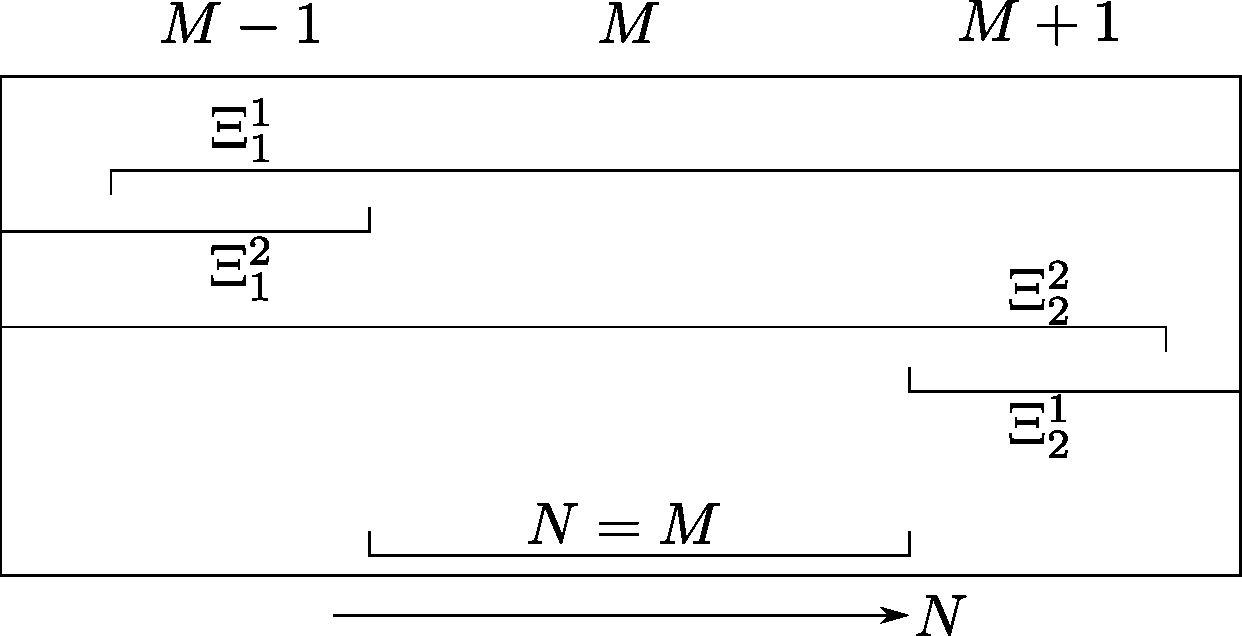
\includegraphics[width=0.7\textwidth]{figures/MNregion}
  \caption{The regions of validity of the functions $\Xi _i ^{(j)}$ of N with respect to M.
    For $N\leq M-1$, $\Xi _i ^{(2)}$ are valid and for $N \geq M+1$, $\Xi _i ^{(1)}$ are valid.
    Only for $N=M$ must the two flavors, $\Xi _i ^{(1)}, \Xi _i ^{(2)}$ mix.}
  \label{fig:mnregion}
\end{figure}

In the local limit $q\to  0$ only certain choices of $m,n$ give non-vanishing results, as is seen from these expressions.
In the case $N=M$, the result always vanishes in the limit.
From Eq. (\ref{eq:15}) we see that the result will be finite only for $N-M-1 = 0$ and $N-M+1=0$, in which case the first factor will be independent of $q$.
One also never gets a negative exponent, which would go to infinity as $q \to 0$, as we will now show.
Consider the upper sign, corresponding to the region $N\geq M+1$ and the flavors $\Xi _i ^{(1)}$.
For the exponent to be negative, $N-M \mp 1 < 0 \implies  N < M \pm 1$, contrary to the region of validity.
In the second region, $N \leq M-1$, corresponding to the lower sing, the criterion $-(N-M \mp 1) < 0 \implies N> M \pm 1$ must hold, but also here the requirement is outside the region of validity.
In conclusion, the overall contribution is \( \delta _{N, M-1} - \delta _{N, M+1} \).

Consider now to the second and third parts of the stress-energy tensor, which are on the form $\Xi _i(\vec{q}, m, n , s) + \Xi _i (\vec{q}, m-1, n-1, s)$, in the local limit.
As the difference $M-N$ does not change under $m\to m-1, n\to n-1$, the exponent of $\widehat{\Xi} _i(q, m-1, n-1)$ is the same as $\widehat{\Xi} _i(q, m, n)$.
Therefore, $\widehat{\Xi} _i(\vec{q}, m, n, s) = \widehat{\Xi} _i(\vec{q}, m-1, n-1, s)$.
It is thus sufficient to check only
\begin{equation}
  \label{eq:23}
  \begin{split}
    (\widehat{\Xi} _1(\vec{q}) + \widehat{\Xi} _2(\vec{q}))
    \widehat{\Xi} _1(\bar{\vec{q}})
      &=
      \begin{multlined}[t]
        \left[ (\mp q_x - iq_y)^{\pm [N-M + 1]} + (\mp q_x - iq_y)^{\pm [N-M-1]} \right]\\
        (\mp q_x + iq_y)^{\pm [N-M + 1]}
      \end{multlined}
      \\
      &= [\qvec{q}^2]^{\pm [N-M+1]} + [\qvec{q}^2]^{\pm [N-M-1]} (\mp q_x + iq_y)^{\pm 2} \right],
  \end{split}
\end{equation}
and
\begin{equation}
  \label{eq:24}
  \begin{split}
    (\widehat{\Xi} _1(\vec{q}) + \widehat{\Xi} _2(\vec{q}))
    \widehat{\Xi} _2(\bar{\vec{q}})
      &=
      \begin{multlined}[t]
        \left[ (\mp q_x - iq_y)^{\pm [N-M + 1]} + (\mp q_x - iq_y)^{\pm [N-M-1]} \right]\\
        (\mp q_x + iq_y)^{\pm [N-M - 1]}
      \end{multlined}
      \\
      &= [\qvec{q}^2]^{\pm [N-M-1]} \left[ (\mp q_x - iq_y )^{\pm 2} +  1 \right].
  \end{split}
\end{equation}
Similar reasoning as above may be applied to Eqs. (\ref{eq:23}) and (\ref{eq:24}).
We get the selection rules \( N = M - 1, N= M+1 \), respectively.

Consequently, when taking the matrix elements $J^x_{\vec{k} ms, \vec{k}+\vec{q}ns} T^{0y \; (i)}_{\vec{k}+\vec{q}ns, \vec{k}ms}$, only certain combinations of the $\Xi_j$-functions will give finite contributions.
The surviving contributions are summarized as follows, where prefactors are omitted to highlight the structure and signs of the  terms,
\begin{align*}
  J^x_{\vec{k} ms, \vec{k}+\qvec{q}ns} T^{0y \; (1)}_{\vec{k}+\qvec{q}ns, \vec{k}ms}
  &: \Xi_{1} (\vec{q}, m,n,s) \Xi_1 (\bar{\vec{q}}, m, n, s) \delta _{N, M-1} - \Xi_{2} (\vec{q}, m,n,s) \Xi_2 (\bar{\vec{q}}, m, n, s) \delta _{N, M+1},\\
  J^x_{\vec{k} ms, \vec{k}+\qvec{q}ns} T^{0y \; (2)}_{\vec{k} + \qvec{q}ns, \vec{k}ms}
  &:  \Xi_{1} (\vec{q}, m,n,s) \left[
    \Xi_{1} (\bar{\vec{q}}, m, n, s) + \Xi _1 (\bar{\vec{q}}, m-1, n-1, s)
  \right] \delta _{N, M-1},\\
  J^x_{\vec{k} ms, \vec{k}+\qvec{q}ns} T^{0y \; (3)}_{\vec{k}+\qvec{q}ns, \vec{k}ms}
  &: \Xi_{2} (\vec{q}, m,n,s) \left[
    \Xi_{2} (\bar{\vec{q}}, m, n, s) + \Xi _2 (\bar{\vec{q}}, m-1, n-1, s)
  \right] \delta _{N, M+1}.\\
\end{align*}

\subsubsection{Final form of response function}
It is now finally possible to write out the entire response function.
The response function will be split into three parts, $\chi ^{xy\; (i)},\: i = 1,2,3$ corresponding to the three parts of the stress-energy tensor.
Also, the sum over the $\vec{k}$ values will be replaced by an integral.
Firstly, we will show that the sum over $k_x$ is restricted;
recall that the eigenfunctions are exponentially centered around $y_0 = k_x l_B^2$, which for a finite sample we expect to be restricted to $0 \leq y_0 \leq L_y$.
This restricts the $k_x$ sum to $0 \leq k_x \leq L_y / l_B^2 = L_ye B /\hbar $, resulting in the $k_x$ summation giving a finite degeneracy contribution~\cites[Ch.~1.4.1]{tongGaugeTheoryLecture}{linderIntermediateQuantumMechanics2017}.
\begin{align}
  \sum\limits_{\vec{k}}^{} = \sum\limits_{k_x = 0}^{L_y eB / \hbar } \sum\limits_{k_z}^{} &\to 
                                                                                            \frac{L_xL_z}{(2\pi )^2} \int\limits_0^{L_y e B /\hbar } \mathrm{d}k_x \int\mathrm{d}k_z \\
  &= \frac{\mathcal{V} e B}{(2 \pi)^2 \hbar } \int \mathrm{d}k_{z}.
\end{align}
Recall the response function
\begin{equation}
  \chi ^{xy} (\omega , \vec{q}) =
  \lim_{\eta \to 0}
  \sum\limits_{\vec{k}, mn}^{}
  \frac{1}{\mathcal{V}}
  \frac{
    i v_F \hbar J^x_{\vec{k} m s, \vec{k}+\qvec{q} n s}(\vec{q})
    T^{0y}_{\vec{k}+\qvec{q} ns, \vec{k}ms}(\vec{q})
    \;
    [n_{\vec{k} m s}- n_{\vec{k}+\qvec{q} ns }]
  }{
    (E_{\vec{k} m s} - E_{\vec{k} + \qvec{q} ns} + i \hbar  \eta )
    (E_{\vec{k} m s} - E_{\vec{k} + \qvec{q} ns} + \hbar \omega + i \hbar  \eta )
  }
  .
\end{equation}
Splitting up the stress-energy tensor, and considering each part of the response function by itself, as explained above, gives

\begin{equation}
  \begin{split}
    \chi ^{xy \; (i)}(\omega , \vec{q}) &=
    \begin{multlined}[t]
      \lim_{\eta \to 0}
      \frac{eB i v_F \hbar  }{\hbar (2\pi)^2 }
      \sum\limits_{mn}^{} 
      \int \mathrm{d}k_z
      [n_{\vec{k} ms} - n_{\vec{k}+\qvec{q} ns}]\\
      \frac{
        J^x_{\vec{k}ms, \vec{k}+\qvec{q} ns}(\vec{q})
        T^{0y\; (i)}_{\vec{k}+\qvec{q}ns, \vec{k}ms}(\vec{q})
      }{
        (E_{\vec{k} m s} - E_{\vec{k} + \qvec{q} ns} + i \hbar  \eta )
        (E_{\vec{k} m s} - E_{\vec{k} + \qvec{q} ns} + \hbar \omega + i \hbar  \eta )
      }
    \end{multlined}\\
    &=
    \begin{multlined}[t]
      \lim_{\eta \to 0}
      \frac{ -e^2 B v_F^2 s
        \Gamma ^-_{\vec{k} \qvec{q} m n s}
        \Gamma ^+_{\vec{k} \qvec{q} m n s}
      }{4 (2\pi )^2}
      \sum\limits_{mn}^{}  
      \int \mathrm{d}k_z\\
      \frac{
        (\Xi _1 + \Xi _2)
        \left( \dots  \right)^i
        [n_{\vec{k} ms} - n_{\vec{k}+\qvec{q} ns}]
      }{
        (E_{\vec{k} m s} - E_{\vec{k} + \qvec{q} ns} + i \hbar  \eta )
        (E_{\vec{k} m s} - E_{\vec{k} + \qvec{q} ns} + \hbar \omega + i \hbar  \eta )
      },
    \end{multlined}
  \end{split}
\end{equation}
where

\begin{align}
  (\dots )^1 &= s(E_{\vec{k} m s} + E_{\vec{k} + \qvec{q} ns} - 2\mu ) (\Xi _{1} (\bar{\vec{q}}, m, n, s) - \Xi _2(\bar{\vec{q}}, m, n, s)),\\
  (\dots)^2 &= \frac{\hbar v_F}{l_B}
                                                           \left\{
                                                             \frac{\sqrt{2M}}{\alpha _{\vec{k} m s} }
                                                             \Xi_1(\bar{\vec{q}}, m, n, s)
                                                             \right.
                                                             \left.+
                                                             \sqrt{2(M-1)}
                                                             \frac{\alpha _{\vec{k} m s} \alpha _{\vec{k} + \qvec{q} n s}}{\alpha _{\vec{k} m-1 s}}
                                                             \Xi_1(\bar{\vec{q}}, m-1, n -1, s)
                                                           \right\},\\
  (\dots )^3 &= \frac{\hbar  v_F}{l_B}
                                                           \left\{
                                                             \frac{\sqrt{2 N} }{\alpha _{\vec{k} + \qvec{q} n s}}
                                                             \Xi _2(\bar{\vec{q}}, m, n, s)
                                                             \right.
                                                             \left.+
                                                             \sqrt{2(N-1)}
                                                             \frac{\alpha _{\vec{k} m s} \alpha _{\vec{k} + \qvec{q} n s}}{\alpha _{\vec{k} + \qvec{q} n-1 s}}
                                                             \Xi _2(\bar{\vec{q}}, m-1, n-1, s)
                                                           \right\}.
\end{align}
In the interest of facilitating for the integration over $k_z$, make a change of variables in the integration, by introducing the dimensionless quantity $\kappa_z = \hbar  k_z /\sqrt{2 e B \hbar }$, which also normalizes the energy to $E_{\vec{k} m s} = v_F \sqrt{2 e B \hbar } \mathcal{\epsilon}_{\kappa _z m s}$, which is seen directly from the expression of the energy eigenvalues.
After some cleaning up, among other taking the product $\Gamma ^-_{\vec{k}\qvec{q} m n s} \Gamma ^+_{\vec{k}\qvec{q} m n s}$ and using $l_B = \sqrt{\hbar /(e B)}$,
\begin{equation}
  \chi ^{xy\; (i)} (\omega , \vec{q}) =
  \lim_{\eta \to 0}
  \frac{-1}{4(2\pi )^2}
  \frac{e^2 B s v_F}{\hbar }
  e^{-\frac{l_B^2}{2} q^2}
  \sum\limits_{mn}^{}
  \int \mathrm{d} \kappa _z
  \xi(\kappa_z)
  \left( \Xi _1  + \Xi _2 \right)
  \Delta ^i,
\end{equation}
where we defined
\begin{equation}
  \xi(\kappa_z) = \frac{[n_{\kappa ms} - n_{\kappa + \qvec{q} ns}]
  \left[ (\alpha _{\kappa ms}^2 + 1) (\alpha _{\kappa +\qvec{q} ns}^2 + 1) \right]^{-1}
  }{
    (\epsilon _{\kappa m s} - \epsilon _{\kappa +\qvec{q}ns} + i \frac{\hbar  \eta }{v_F\sqrt{2 e B \hbar }})
    (\epsilon _{\kappa m s} - \epsilon _{\kappa +\qvec{q}ns} + \frac{\hbar \omega }{v_F \sqrt{2 e B \hbar }} + i \frac{\hbar  \eta }{v_F\sqrt{2 e B \hbar }})
  }
\end{equation}
and
\begin{align}
  \Delta ^1 &= s (\epsilon _{\vec{\kappa} + m + s} + \epsilon _{\vec{\kappa} + \qvec{\vec{q}} ns} - 2 \frac{\hbar \mu }{v_F \sqrt{2eB\hbar }}) (\Xi _1(\bar{\vec{q}}, m, n, s) - \Xi _2 (\bar{\vec{q}}, m, n, s)),\\
  \Delta ^2 &= 
              \frac{\sqrt{M}}{\alpha _{\vec{k} m s} }
              \Xi_1(\bar{\vec{q}}, m, n, s)
              +
              \sqrt{(M-1)}
              \frac{\alpha _{\vec{k} m s} \alpha _{\vec{k} + \qvec{q} n s}}{\alpha _{\vec{k} m-1 s}}
              \Xi_1(\bar{\vec{q}}, m-1, n -1, s),\\
  \Delta^3 &= 
             \frac{\sqrt{ N} }{\alpha _{\vec{k} + \qvec{q} n s}}
             \Xi _2(\bar{\vec{q}}, m, n, s)
             +
             \sqrt{(N-1)}
             \frac{\alpha _{\vec{k} m s} \alpha _{\vec{k} + \qvec{q} n s}}{\alpha _{\vec{k} + \qvec{q} n-1 s}}
             \Xi _2(\bar{\vec{q}}, m-1, n-1, s).
\end{align}
Considering now the local limit $q\to 0$, and using the previously found selection rules for products of the $\Xi _i$-functions.
Using that the Laguerre polynomials are unity at the origin and writing out the $\Xi $-functions with the selection rules
\begin{align}
  \label{eq:46}
  \lim_{\vec{q}\to 0} \chi ^{xy\; (1)} (\omega , \vec{q}) &=
                                        \lim_{\eta \to 0} \frac{1}{4(2\pi )^2}
                                        \frac{e^2 B v_F}{\hbar }
                                        \sum\limits_{mn}
                                        \int \mathrm{d}\kappa _z
  \xi(\kappa _z)
  (\epsilon _{\vec{\kappa}  m  s} + \epsilon _{\vec{\kappa} ns} - 2 \frac{\hbar \mu }{v_F \sqrt{2eB\hbar }})
 (\alpha _{\kappa n s}^2 \delta _{N, M+1} - a_{\kappa m s}^2 \delta _{N, M-1}) ,\\
  \label{eq:47}
  \lim_{\vec{q}\to 0} \chi ^{xy\; (2)} (\omega , \vec{q}) &=
                                        \lim_{\eta \to 0} \frac{1}{4(2\pi )^2}
                                        \frac{e^2 B s v_F}{\hbar }
                                        \sum\limits_{\substack{mn\\ \mathclap{N= M-1}}}
                                        \int \mathrm{d}\kappa _z
                                        \xi(\kappa_z)
                                        \left\{
                                          \sqrt{M} \alpha _{\vec{\kappa } m s}
                                          +
                                          \sqrt{M-1} \alpha _{\vec{\kappa } n s} \alpha _{\vec{\kappa } ms}^2
                                        \right\},\\
  \label{eq:48}
  \lim_{\vec{q}\to 0} \chi ^{xy\; (3)} (\omega , \vec{q}) &=
                                        \lim_{\eta \to 0} \frac{-1}{4(2\pi )^2}
                                        \frac{e^2 B s v_F}{\hbar }
                                        \sum\limits_{\substack{mn\\ \mathclap{N= M+1}}}
                                        \int \mathrm{d}\kappa _z
                                        \xi(\kappa_z)
                                        \left\{
                                          \sqrt{N} \alpha _{\vec{\kappa } n s}
                                          +
                                          \sqrt{N-1} \alpha _{\vec{\kappa } m s} \alpha _{\vec{\kappa } ns}^2
                                        \right\}.
\end{align}
The function \( \xi \) is odd under interchange of \( m,n \), i.e. \( \xi_{m,n} = -\xi _{n,m} \).
Using this, we may simplify our expressions some.
Firstly, in the second term of Eq. \eqref{eq:46}, we may relabel \( m \leftrightarrow n \), and using that \( \xi  \) is odd to get twice the first term.
Doing a similar trick for Eq. \eqref{eq:47} renders it identical to Eq. \eqref{eq:48}.
In total, we get
\begin{align}
  \lim_{\vec{q}\to 0} \chi ^{xy\; (1)} (\omega , \vec{q}) &=
                                        \lim_{\eta \to 0} \frac{1}{4(2\pi )^2}
                                        \frac{e^2 B v_F}{\hbar }
                                        \sum\limits_{\substack{mn\\ \mathclap{N=M+1}}}
                                        \int \mathrm{d}\kappa _z
  2 \xi(\kappa _z)
  (\epsilon _{\vec{\kappa}  m  s} + \epsilon _{\vec{\kappa} ns} - 2 \frac{\hbar \mu }{v_F \sqrt{2eB\hbar }})
 \alpha _{\kappa n s}^2 ,\\
  \lim_{\vec{q}\to 0} \chi ^{xy\; (2,3)} (\omega , \vec{q}) &=
                                        \lim_{\eta \to 0} \frac{-1}{4(2\pi )^2}
                                        \frac{e^2 B s v_F}{\hbar }
                                        \sum\limits_{\substack{mn\\ \mathclap{N= M+1}}}
                                        \int \mathrm{d}\kappa _z
                                        2 \xi(\kappa_z)
                                        \left\{
                                          \sqrt{N} \alpha _{\vec{\kappa } n s}
                                          +
                                          \sqrt{N-1} \alpha _{\vec{\kappa } m s} \alpha _{\vec{\kappa } ns}^2
                                        \right\}.
\end{align}
Here, \( \chi ^{xy\; (2,3)} = \chi ^{xy\; (2)} + \chi ^{xy\; (3)} \).

Note the $\alpha _{\kappa ns}$ factors coming from the $\Xi $ functions;
it is also important to note that the latter term involves the chirality $s$, which is of concern as this could make pairs of nodes cancel, however, we will see that the term ends up not being dependent on $s$.
In the static limit $\lim_{\omega \to 0}$ and with the potential $\mu =0$ the integral may be solved.
Including only the lowest Landau level contribution, that is, the sum restricted to $m=0, n=\pm 1$, the contributions were found to be
\begin{align}
  \lim_{\omega \to  0} \lim_{\vec{q}\to 0}
  \chi ^{xy \; (1)}
  &= \frac{1}{2} \frac{e^2B v_F}{4 (2\pi )^2 \hbar },\\
  \lim_{\omega \to  0} \lim_{\vec{q}\to 0}
  \chi ^{xy \; (3)}
  &= \frac{1}{2} \frac{e^2B s^2 v_F}{4 (2\pi )^2 \hbar }.
\end{align}
For clarity $s^2$ was included explicitly, showing that the aforementioned $s$-dependence is not an issue.
The total transverse response function with only first level contributions is therefore
\begin{equation}
  \lim_{\omega \to  0} \lim_{\vec{q}\to 0}
  \chi ^{xy}
  = \frac{e^2B v_F}{4 (2\pi )^2 \hbar }.
\end{equation}
Including higher order contributions, only gives additional numerical prefactors,
\begin{equation}
 \label{eq:34} 
  \lim_{\omega \to  0} \lim_{\vec{q}\to 0}
  \chi ^{xy}
  = \gamma_M \frac{e^2B v_F}{4 (2\pi )^2 \hbar },
\end{equation}
with $\gamma _0 = 1, \gamma _{20} \approx 2$, and where $\gamma _M$ goes as $\log M$.
The first 300 contributions were calculated, shown in Figure \ref{fig:convergence_chi}.


% \todo{Make sure have notes that consider zero T for the distribution}
% In the static limit $\omega \to 0$, with potential $\mu =0$ \todo{explain}, the integral was solved in a CAS \todo{how to formulate this?}, and found to be $\frac{1}{2}$.
% Thus, considering only the lowest Landau level contributions, in which case the sum goes over $n=\pm 1, m=0$ only,
% \begin{equation}
%   \lim_{\omega \to  0} \lim_{\vec{q}\to 0}
%   \chi ^{xy \; (1)}
%   = \frac{e^2B v_F}{4 (2\pi )^2 \hbar }.
% \end{equation}
% Once again, in  the limit the integral is evaluated and found to be $\mp \frac{1}{2}$ for $s=\pm 1$, or rather $- s \frac{1}{2}$.
% Thus, summing over only the two main contributions
% \begin{equation}
%   \lim_{\omega \to  0} \lim_{\vec{q}\to 0}
%   \chi ^{xy \; (3)}
%   = \frac{e^2B s^2 v_F}{4 (2\pi )^2 \hbar }.
% \end{equation}
% The total transverse response function is therefore
% \begin{equation}
%   \lim_{\omega \to  0} \lim_{\vec{q}\to 0}
%   \chi ^{xy}
%   = \frac{e^2B v_F}{2 (2\pi )^2 \hbar }.
% \end{equation}

\begin{figure}[h]
  \centering
  \input{figures/convergence_chi}
  \caption{Prefactor $\gamma_N$ of $\chi$ vs. number of terms $N$ included in sum.}
  \label{fig:convergence_chi}
\end{figure}


\section{Discussion of results}
In the static and local limit $\lim_{\omega \to 0} \lim_{\vec{q}\to 0}$ the  transverse response function $\chi^{xy}$ of the charge current to a temperature perturbation
\begin{equation}\label{eq:44}
  J^x = \chi ^{xy} \frac{- \nabla^y T}{T}
\end{equation}
from a single Dirac point was found  to be
\begin{equation}
  \lim_{\omega \to 0} \lim_{\vec{q}\to 0}
  \chi ^{xy}
  =
  \gamma_{N}
  \frac{e^2 B v_F}{4 (2\pi )^2 \hbar },
\end{equation}
with $\gamma _N$ a prefactor dependent on how many landau levels are included in the final evaluation of the response function.
The response function is independent of the chirality $s$ of the Dirac point.
It was found that $\gamma _0 = 1, \gamma _{20} \approx 2$ and that the prefactor goes like $\log N$.

Firstly, the result differ slightly from that found by~\citeauthor{arjonaFingerprintsConformalAnomaly2019} ~\cite{arjonaFingerprintsConformalAnomaly2019}
\begin{equation}
  \lim_{\omega \to 0} \lim_{\vec{q}\to 0}
  \chi ^{xy}
  =
  2 \gamma_{N}
  \frac{e^2 B v_F}{4 (2\pi )^2 \hbar },
\end{equation}
which differ by a factor of two.

Secondly, the sum will diverge as $N\to \infty $.
However, not all Landau levels are filled, and thus the sum should not be taken to all levels.
Similarly to a Quantum Hall effect, the number of filled bands, the filling factor $\nu $, is inverse proportional to the $B$-field strength
\begin{equation}
  \nu \propto \frac{1}{B}.
\end{equation}
Thus, we expect that the $N$-sum should be truncated at a Landau level, given by the filling factor $\nu $.
A detailed derivation of the exact truncation of the $N$-sum has not been done.
If a precise result for the numerical prefactor is found to be of importance, this should be straightforward.

The divergence is not discussed by~\citeauthor{arjonaFingerprintsConformalAnomaly2019}, where only the values of $N = 0$ and  $N=20$ are given, and the final result is that of $N=20$.
Furthermore, they state that the contributions from higher values of $N$ decrease very rapidly.
However, we found the contributions to go like $1 /x$, which is not decreasing rapidly enough to give a finite total contribution, thus giving the total contribution diverging logarithmically.
\todo{Say that we are communicating with them  to better understand their chioce of truncation?}
Comparing our result with the different procedure done by~\citeauthor{chernodubGenerationNernstCurrent2018}~\cite{chernodubGenerationNernstCurrent2018}, the numerical prefactor found in our calculation including only the first term ($M=0$) coincides very well with the numerical prefactor found there, with a ratio of $16 / 18$.
